\documentclass{article}
\usepackage[utf8]{inputenc}
\usepackage[english]{babel}
\usepackage{listings}
\usepackage{bytefield}
\usepackage{xcolor}
\usepackage{tikz}
\usepackage{pgf-umlsd}
\usepackage{afterpage}
\usepackage{hyperref}
\usetikzlibrary{automata, positioning, arrows}

\definecolor{lightgray}{gray}{0.8}

\tikzset{->,  
         >=stealth',
         node distance=6cm, 
         every state/.style={thick, fill=gray!10},
         initial text=$ $,
         }
         
\newenvironment*{returnanother}[6][1]{
  \stepcounter{seqlevel}
  \stepcounter{callevel} % push
  \path
  (#2)+(0,-\theseqlevel*\unitfactor-0.7*\unitfactor) node (cf\thecallevel) {}
  (#4.\threadbias)+(0,-\theseqlevel*\unitfactor-0.7*\unitfactor) node (ct\thecallevel) {};
  \draw[->,>=triangle 60] ({cf\thecallevel}) -- (ct\thecallevel)
  node[midway, above] {#3};
  \def\l\thecallevel{#1}
  \def\f\thecallevel{#6}
  \def\t\thecallevel{#4}
  \def\returnvalue{#5}
  \tikzstyle{threadstyle}+=[instcolor#2]
    \addtocounter{seqlevel}{1}
  \path
  (\f\thecallevel)+(0,-\theseqlevel*\unitfactor-0.7*\unitfactor) node (rf\thecallevel) {}
  (\t\thecallevel.\threadbias)+(0,-\theseqlevel*\unitfactor-0.7*\unitfactor) node (rt\thecallevel) {};
  \draw[dashed,->,>=angle 60] ({rt\thecallevel}) -- (rf\thecallevel)
  node[midway, above]{\returnvalue};
  \drawthread{ct\thecallevel}{rt\thecallevel}
}
{
\addtocounter{seqlevel}{\thecallevel}
%   \path
%   (\f\thecallevel.\threadbias)+(0,-\theseqlevel*\unitfactor+\unitfactor+\l\thecallevel*\unitfactor-0.7*\unitfactor) node (rrf\thecallevel) {}
%   (\f\thecallevel.\threadbias)+(0,-\theseqlevel*\unitfactor-0.7*\unitfactor) node (rff\thecallevel) {};
%  \drawthread{rrf\thecallevel}{rff\thecallevel}
  \addtocounter{callevel}{-1} % pop
  \addtocounter{seqlevel}{-1}
}

\begin{document}

\tableofcontents

\section{Memory donation}

\subsection{Scheduler $\rightarrow$ secondary VM}
Initially, VM 0 has both ownership and exclusive access to pages $p_1$, $p_2$. After a complete donation transaction, it loses ownership and access to these pages and passes it to VM 1.

More precisely, VM 0 initiates a memory donation transaction by populating a memory transaction descriptor (within its TX buffer) with receivers' IDs, PIDs, and some auxiliary information. R0 is populated with a function id of FFA\_MEM\_DONATE, R1 is populated with a length of a memory descriptor. FFA\_MEM\_DONATE returns a handle for this transaction. At this point, VM 0 still owns the pages, however, it loses access to it. After the transaction initiation, VM 0 populates the memory transaction descriptor with the handle, and sends it via FFA\_MSG\_SEND (perhaps, without its endpoint array), and transfers control to VM 1. VM 1 copies the memory transaction descriptor from its RX to TX buffer, and finishes the transaction by calling FFA\_MEM\_RETRIEVE. After that, VM 1 has both ownership and exclusive access to the pages.

\subsubsection{Bare-bones version}

Assumptions:
\begin{enumerate}
 \item VM 0 owns pages $p_1$, $p_2$ and has exclusive access to it.
 \item VM 0 owns its TX buffer, RX buffer of VM 1 is empty.
 \item The following memory slice of the scheduler's TX buffer is valid: \\
     \\
     \begin{bytefield}[rightcurly=., rightcurlyspace=0pt, bitwidth=1.2em]{16}
         \bitheader[endianness=little]{0,2,3,4,8,16} \\
         \begin{rightwordgroup}{n}
             \bitbox{2}{0x0}
	         \bitbox{1}[bgcolor=lightgray]{}
	         \bitbox{1}[bgcolor=lightgray]{}
	         \bitbox{4}{0x0}
	         \bitbox{8}{0x0}
         \end{rightwordgroup} \\
         \begin{rightwordgroup}{n + 0x10}
             \bitbox{8}[bgcolor=lightgray]{}
	         \bitbox{4}[bgcolor=lightgray]{}
	         \bitbox{4}{0x1}
         \end{rightwordgroup} \\
         \begin{rightwordgroup}{n + 0x20}
             \bitbox{2}{0x1}
             \bitbox{1}[bgcolor=lightgray]{}
             \bitbox{1}[bgcolor=lightgray]{}
             \bitbox{4}{m - n}
             \bitbox{8}[bgcolor=lightgray]{}
         \end{rightwordgroup} \\
         \skippedwords \\
         \begin{rightwordgroup}{m}
             \bitbox{4}{0x2}
             \bitbox{4}{0x2}
             \bitbox{8}[bgcolor=lightgray]{}
         \end{rightwordgroup} \\
         \begin{rightwordgroup}{m + 0x10}
             \bitbox{8}{addr(p1)}
             \bitbox{4}{0x1}
             \bitbox{4}[bgcolor=lightgray]{}
         \end{rightwordgroup} \\
         \begin{rightwordgroup}{m + 0x20}
             \bitbox{8}{addr(p2)}
             \bitbox{4}{0x1}
             \bitbox{4}[bgcolor=lightgray]{}
         \end{rightwordgroup}
     \end{bytefield}
\end{enumerate}

\begin{lstlisting}[caption={VM 0}]
# memory donation ffa call
mov R0, 0x84000071 # function id (FFA_MEM_DONATE)
mov R1, 0x30       # Total length of the memory transaction 
                   # descriptor in bytes
mov R2, 0x30       # Length in bytes of the memory transaction 
                   # descriptor passed in this ABI invocation
                   # (it's possible to split it in a number of fragments)
mov R3, 0x0        # (base address of a buffer) used if 
                   # transaction descriptor is sent in 
                   # dynamically allocated buffers, mbz otherwise
mov R4, 0x0        # (number of 4K pages in a buffer) used if 
                   # transaction descriptor is sent in 
                   # dynamically allocated buffers, mbz otherwise
mov R5, 0x0        # mbz
mov R6, 0x0        # mbz
mov R7, 0x0        # mbz
hvc

# R3 is populated with the page handler at this point

# we need to inform VM 1 of the handler by sending an indirect message
mov R0, 0x8400006E # function id (FFA_MSG_SEND)

# Bit[31:16]: Sender endpoint ID.
# Bit[15:0]: Receiver endpoint ID.
# In this case, it's redundant, however, it's kept as an example
mov R1, 0x0
mov R1, R1, LSL 16
add R1, 0x1        # callee id
mov R4, addr(TX)
str R2, [R4, 8]    # store the handler in TX_0_1 buffer of VM0
str R3, [R4, 12]
hvc

mov R0, 0x8400006D # function id (FFA_RUN)
# Bit[31:16]: Callee ID.
# Bit[15:0]: Callee vCPU ID.
mov R1, 0x1        # callee id
mov R1, R1, LSL 16
add R1, 0x0        # vCPU id
hvc
\end{lstlisting}

\begin{lstlisting}[caption={VM 1}]
# Copy RX to TX

mov R0, 0x84000074 # function id (FFA_MEM_RETRIEVE_REQ)
mov R1, 0x30       # Total length of the memory transaction 
                   # descriptor in bytes
mov R2, 0x30       # Length in bytes of the memory transaction 
                   # descriptor passed in this ABI invocation
                   # (it's possible to split it in a number of fragments)
mov R3, 0x0        # (base address of a buffer) used if 
                   # transaction descriptor is sent in 
                   # dynamically allocated buffers, mbz otherwise
mov R4, 0x0        # (number of 4K pages in a buffer) used if 
                   # transaction descriptor is sent in 
                   # dynamically allocated buffers, mbz otherwise
mov R5, 0x0        # mbz
mov R6, 0x0        # mbz
mov R7, 0x0        # mbz
hvc

mov R0, 0x8400006C # function id (FFA_YIELD)
mov R1, 0x0        # mbz
mov R2, 0x0        # mbz
mov R3, 0x0        # mbz
mov R4, 0x0        # mbz
mov R5, 0x0        # mbz
mov R6, 0x0        # mbz
mov R7, 0x0        # mbz
hvc
\end{lstlisting}

\subsubsection{OpSem version}

\begin{figure}[hbt!]
\centering
\begin{sequencediagram}
    \newinst{Hyp}{Hypervisor}
    \newinst[3]{VM0}{VM 0}
    \newinst[3]{VM1}{VM 1}
    
    \begin{call}{VM0}{MEM\_DONATE (1)}{Hyp}{SUCCESS}
    \end{call}
    
    \begin{call}{VM0}{MSG\_SEND (1)}{Hyp}{SUCCESS}
    \end{call}
    
    \begin{returnanother}{VM0}{RUN (1)}{Hyp}{}{VM1}    
        \begin{call}{VM1}{MSG\_WAIT}{Hyp}{MSG\_SEND}
        \end{call}
        
        \begin{call}{VM1}{MEM\_RETRIEVE\_REQ}{Hyp}{MEM\_RETRIEVE\_RESP}
        \end{call}
    \end{returnanother}
    
    \begin{returnanother}{VM1}{YIELD}{Hyp}{}{VM0}
    \end{returnanother}
        
\end{sequencediagram}
\end{figure}

\begin{figure}[hbt!]
\centering
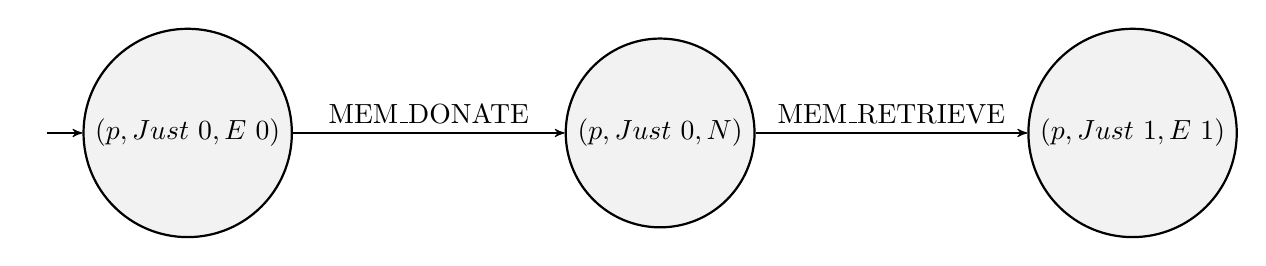
\begin{tikzpicture}
    \node[state, initial] (q1) {$(p, Just\ 0, E\ 0)$};
    \node[state, right of=q1] (q2) {$(p, Just\ 0, N)$};
    \node[state, right of=q2] (q3) {$(p, Just\ 1, E\ 1)$};
    
    \draw   (q1) edge[above] node{MEM\_DONATE} (q2)
            (q2) edge[above] node{MEM\_RETRIEVE} (q3);
\end{tikzpicture}
\end{figure}

\begin{lstlisting}[caption={VM 0}]
# save 42
mov R0, addr(p, 0)              # p address
mov R1, 42                      # payload
str R0, R1                      # write payload to p

# mem_donate
# arguments
mov R0, encode_fid(MEM_DONATE)  # function id (FFA_MEM_DONATE)
mov R1, 6                       # Total length of the  
                                # memory transaction descriptor
# VMID of the sender 
mov R2, addr(tx, 0)             # TX buffer address                               
mov R3, 0
str R2, R3

# flag
mov R2, addr(tx, 1)             # TX buffer address (offset 1)                               
mov R3, 0                       # not zeroed
str R2, R3

# handle (mbz)
mov R2, addr(tx, 2)             # TX buffer address (offset 2)
mov R3, 0
str R2, R3

# tag (extra information)
mov R2, addr(tx, 3)             # TX buffer address (offset 3)
mov R3, 0
str R2, R3

# access descriptor count (must be 1 for donation)
mov R2, addr(tx, 4)             # TX buffer address (offset 4)
mov R3, 1
str R2, R3

# VMID of the receiver
mov R2, addr(tx, 5)             # TX buffer address (offset 5)
mov R3, 1
str R2, R3

# base address of the donated page
mov R2, addr(tx, 6)             # TX buffer address (offset 6)
mov R3, addr(p, 0)              # p address
str R2, R3

hvc            # [0].pt[p] = (O, NA)
               # [1].pt[p] = (!O, NA)
               # sss[handler] = (0, flag, tag, inl (1, p), MEM_DONATE)

# R2 is populated with the transaction discriptor at this point
# save it to the discriptor
mov R3, addr(tx, 2)             # TX buffer address (offset 2)
str R3, R2

# msg_send
mov R0, encode_fid(MSG_SEND)    # function id (FFA_MSG_SEND)
mov R1, 1                       # VMID of the receiver
mov R2, 6                       # message length
hvc

# run
mov R0, encode_fid(FFA_RUN)
mov R1, 1
hvc
\end{lstlisting}

\begin{lstlisting}[caption={VM 1}]
# retrieve msg length
mov R0, encode_fid(MSG_WAIT)    # function id (FFA_MSG_WAIT)
hvc

# R1 is populated with length of the message at this point

# Copy RX to TX
mov R0, 0             # value to compare with
mov R2, loop          # jump point
mov R3, 1             # step
mov R4, addr(rx, 0)   # RX buffer base address
mov R5, addr(tx, 0)   # TX buffer base address
loop:
sub R1, R1, R3
cmp R1, R0
ldr R6, R4
str R5, R6
add R4, R4, R3
bne R2

mov R0, encode_fid(MEM_RETRIEVE_REQ) # function id (FFA_MEM_RETRIEVE_REQ)
mov R1, 4                            # Total length of the  
                                     # memory transaction descriptor in bytes
# access descriptor count (must be 0 for mem_retrieve)
mov R2, addr(tx, 4)           # TX buffer address (offset 4)
mov R3, 0
str R2, R3                                    
hvc               # [0].pt[p] = (!O, NA)
                  # [1].pt[p] = (O, EA)
                  # find(sss, handler) = False
                  
# yield
mov R0, encode_fid(YIELD)     # function id (FFA_YIELD)
hvc
\end{lstlisting}

\subsection{Secondary VM $\rightarrow$ secondary VM}
Initially, VM 1 has both ownership and exclusive access to pages $p_1$, $p_2$. After a complete donation transaction, it loses ownership and access to these pages and passes it to VM 2.

More precisely, VM 0 (scheduler) gives control to VM 1. VM 1 initiates a memory donation transaction by populating a memory transaction descriptor (within its TX buffer) with receivers' IDs, PIDs, and some auxiliary information. R0 is populated with a function id of FFA\_MEM\_DONATE, R1 is populated with a length of a memory descriptor. FFA\_MEM\_DONATE returns a handle for this transaction. At this point, VM 1 loses access to the pages, however, it still owns the pages. After the transaction initiation, VM 1 populates the memory transaction descriptor with the handle, and sends it via FFA\_MSG\_SEND (perhaps, without endpoint array), and consequently yields control to VM 0. VM 0 simply gives control to VM 2. After that, VM 2 copies the memory transaction descriptor from RX to TX buffer, and finishes the transaction by calling FFA\_MEM\_RETRIEVE. Both ownership and exclusive access over $p_1$ and $p_2$ now belong to VM 2.

\subsubsection{Bare-bones version}
Assumptions:
\begin{enumerate}
 \item VM 1 owns pages $p_1$, $p_2$ and have exclusive access to it.
 \item VM 1 owns its TX buffer, RX buffer of VM 2 is empty.
 \item The following memory slice of the TX buffer is valid: \\
     \\
     \begin{bytefield}[rightcurly=., rightcurlyspace=0pt, bitwidth=1.2em]{16}
         \bitheader[endianness=little]{0,2,3,4,8,16} \\
         \begin{rightwordgroup}{n}
             \bitbox{2}{0x1}
	         \bitbox{1}[bgcolor=lightgray]{}
	         \bitbox{1}[bgcolor=lightgray]{}
	         \bitbox{4}{0x0}
	         \bitbox{8}{0x0}
         \end{rightwordgroup} \\
         \begin{rightwordgroup}{n + 0x10}
             \bitbox{8}[bgcolor=lightgray]{}
	         \bitbox{4}[bgcolor=lightgray]{}
	         \bitbox{4}{0x1}
         \end{rightwordgroup} \\
         \begin{rightwordgroup}{n + 0x20}
             \bitbox{2}{0x2}
             \bitbox{1}[bgcolor=lightgray]{}
             \bitbox{1}[bgcolor=lightgray]{}
             \bitbox{4}{m - n}
             \bitbox{8}[bgcolor=lightgray]{}
         \end{rightwordgroup} \\
         \skippedwords \\
         \begin{rightwordgroup}{m}
             \bitbox{4}{0x2}
             \bitbox{4}{0x2}
             \bitbox{8}[bgcolor=lightgray]{}
         \end{rightwordgroup} \\
         \begin{rightwordgroup}{m + 0x10}
             \bitbox{8}{addr(p1)}
             \bitbox{4}{0x1}
             \bitbox{4}[bgcolor=lightgray]{}
         \end{rightwordgroup} \\
         \begin{rightwordgroup}{m + 0x20}
             \bitbox{8}{addr(p2)}
             \bitbox{4}{0x1}
             \bitbox{4}[bgcolor=lightgray]{}
         \end{rightwordgroup}
     \end{bytefield}
\end{enumerate}

\begin{lstlisting}[caption={VM 0}]
# run 1
mov R0, 0x8400006D # function id (FFA_RUN)
# Bit[31:16]: Callee ID.
# Bit[15:0]: Callee vCPU ID.
mov R1, 0x1        # callee id
mov R1, R1, LSL 16
add R1, 0x0        # vCPU id

# run 2
mov R0, 0x8400006D # function id (FFA_RUN)
mov R1, 0x2
mov R1, R1, LSL 16
add R1, 0x0
\end{lstlisting}

\begin{lstlisting}[caption={VM 1}]
# memory donation ffa call
mov R0, 0x84000071 # function id (FFA_MEM_DONATE)
mov R1, 0x30       # Total length of the memory transaction 
                   # descriptor in bytes
mov R2, 0x30       # Length in bytes of the memory transaction 
                   # descriptor passed in this ABI invocation
                   # (it's possible to split it in a number of fragments)
mov R3, 0x0        # (base address of a buffer) used if 
                   # transaction descriptor is sent in 
                   # dynamically allocated buffers, mbz otherwise
mov R4, 0x0        # (number of 4K pages in a buffer) used if 
                   # transaction descriptor is sent in 
                   # dynamically allocated buffers, mbz otherwise
mov R5, 0x0        # mbz
mov R6, 0x0        # mbz
mov R7, 0x0        # mbz
hvc

# R3 is populated with the page handler at this point

# we need to inform VM 1 of the handler by sending an indirect message
mov R0, 0x8400006E # function id (FFA_MSG_SEND)

# Bit[31:16]: Sender endpoint ID.
# Bit[15:0]: Receiver endpoint ID.
mov R1, 0x1
mov R1, R1, LSL 16 # caller id
add R1, 0x2        # callee id
mov R4, addr(TX)
str R2, [R4, 8]    # store the handler in TX buffer of VM 0
str R3, [R4, 12]
hvc
\end{lstlisting}

\begin{lstlisting}[caption={VM 2}]
# Copy RX to TX

mov R0, 0x84000074 # function id (FFA_MEM_RETRIEVE_REQ)
mov R1, 0x30       # Total length of the memory transaction 
                   # descriptor in bytes
mov R2, 0x30       # Length in bytes of the memory transaction 
                   # descriptor passed in this ABI invocation
                   # (it's possible to split it in a number of fragments)
mov R3, 0x0        # (base address of a buffer) used if 
                   # transaction descriptor is sent in 
                   # dynamically allocated buffers, mbz otherwise
mov R4, 0x0        # (number of 4K pages in a buffer) used if 
                   # transaction descriptor is sent in 
                   # dynamically allocated buffers, mbz otherwise
mov R5, 0x0        # mbz
mov R6, 0x0        # mbz
mov R7, 0x0        # mbz
hvc

mov R0, 0x8400006C # function id (FFA_YIELD)
mov R1, 0x0        # mbz
mov R2, 0x0        # mbz
mov R3, 0x0        # mbz
mov R4, 0x0        # mbz
mov R5, 0x0        # mbz
mov R6, 0x0        # mbz
mov R7, 0x0        # mbz
hvc
\end{lstlisting}

\subsubsection{OpSem version}

\begin{figure}[hbt!]
\centering
\begin{sequencediagram}
    \newinst{Hyp}{Hypervisor}
    \newinst[3]{VM0}{VM 0}
    \newinst[3]{VM1}{VM 1}
    \newinst[3]{VM2}{VM 2}
    
    \begin{returnanother}{VM0}{RUN (1)}{Hyp}{}{VM1}  
        \begin{call}{VM1}{MEM\_DONATE (2)}{Hyp}{SUCCESS}
        \end{call}
        \begin{returnanother}{VM1}{MSG\_SEND (2)}{Hyp}{MSG\_SEND}{VM0}
        \end{returnanother}
    \end{returnanother}
    
    \begin{returnanother}{VM0}{RUN (2)}{Hyp}{}{VM2}    
        \begin{call}{VM2}{MSG\_WAIT}{Hyp}{MSG\_SEND}
        \end{call}
        
        \begin{call}{VM2}{MEM\_RETRIEVE\_REQ}{Hyp}{MEM\_RETRIEVE\_RESP}
        \end{call}
        
        \begin{returnanother}{VM2}{YIELD}{Hyp}{}{VM0}
        \end{returnanother}
    \end{returnanother}
        
\end{sequencediagram}
\end{figure}

\begin{figure}[hbt!]
\centering
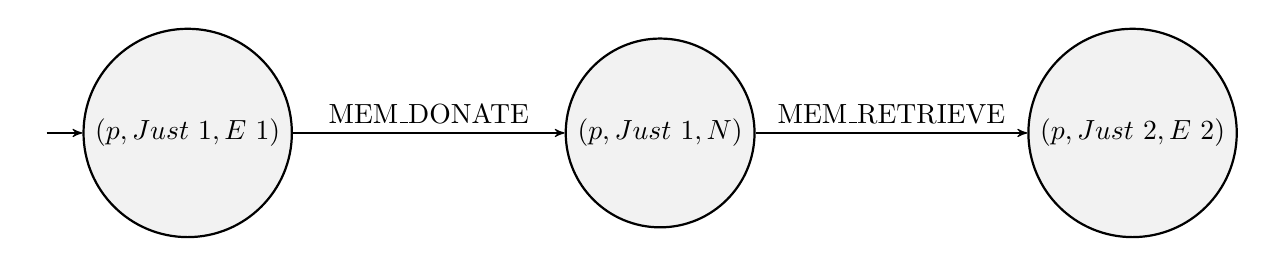
\begin{tikzpicture}
    \node[state, initial] (q1) {$(p, Just\ 1, E\ 1)$};
    \node[state, right of=q1] (q2) {$(p, Just\ 1, N)$};
    \node[state, right of=q2] (q3) {$(p, Just\ 2, E\ 2)$};
    
    \draw   (q1) edge[above] node{MEM\_DONATE} (q2)
            (q2) edge[above] node{MEM\_RETRIEVE} (q3);
\end{tikzpicture}
\end{figure}

\begin{lstlisting}[caption={VM 0}]
# run 1
mov R0, encode_fid(FFA_RUN) # function id (FFA_RUN)
mov R1, 1                   # callee VMID

# run 2
mov R0, encode_fid(FFA_RUN) # function id (FFA_RUN)
mov R1, 2                   # callee VMID
hvc
\end{lstlisting}

\begin{lstlisting}[caption={VM 1}]
# save 42
mov R0, addr(p, 0)              # p address
mov R1, 42                      # payload
str R0, R1                      # write payload to p

# mem_donate
# arguments
mov R0, encode_fid(MEM_DONATE)  # function id (FFA_MEM_DONATE)
mov R1, 6                       # Total length of the  
                                # memory transaction descriptor
# VMID of the sender 
mov R2, addr(tx, 1)             # TX buffer address                               
mov R3, 0
str R2, R3

# flag
mov R2, addr(tx, 1)             # TX buffer address (offset 1)                               
mov R3, 0                       # not zeroed
str R2, R3

# handle (mbz)
mov R2, addr(tx, 2)             # TX buffer address (offset 2)
mov R3, 0
str R2, R3

# tag (extra information)
mov R2, addr(tx, 3)             # TX buffer address (offset 3)
mov R3, 0
str R2, R3

# access descriptor count (must be 1 for donation)
mov R2, addr(tx, 4)             # TX buffer address (offset 4)
mov R3, 1
str R2, R3

# VMID of the receiver
mov R2, addr(tx, 5)             # TX buffer address (offset 5)
mov R3, 2
str R2, R3

# base address of the donated page
mov R2, addr(tx, 6)             # TX buffer address (offset 6)
mov R3, addr(p, 0)              # p address
str R2, R3

hvc               # [0].pt[p] = (!O, NA)
                  # [1].pt[p] = (O, NA)
                  # [2].pt[p] = (!O, NA)
                  # sss[handler] = (1, flag, tag, inl (2, p), MEM_DONATE)

# R2 is populated with the transaction discriptor at this point
# save it to the discriptor
mov R3, addr(tx, 2)             # TX buffer address (offset 2)
str R3, R2

# msg_send
mov R0, encode_fid(MSG_SEND)    # function id (FFA_MSG_SEND)
mov R1, 2                       # VMID of the Receiver
mov R2, 6                       # message length

hvc
\end{lstlisting}

\begin{lstlisting}[caption={VM 2}]
# retrieve msg length
mov R0, encode_fid(MSG_WAIT)   # function id (FFA_MSG_WAIT)
hvc

# R1 is populated with length of the message at this point

# Copy RX to TX
mov R0, 0             # value to compare with
mov R2, loop          # jump point
mov R3, 1             # step
mov R4, addr(rx, 0)   # RX buffer base address
mov R5, addr(tx, 0)   # TX buffer base address
loop:
sub R1, R1, R3
cmp R1, R0
ldr R6, R4
str R5, R6
add R4, R4, R3
bne R2

mov R0, encode_fid(MEM_RETRIEVE_REQ) # function id (FFA_MEM_RETRIEVE_REQ)
mov R1, 4                            # Total length of the  
                                     # memory transaction descriptor in bytes
# access descriptor count (must be 0 for mem_retrieve)
mov R2, addr(tx, 4)             # TX buffer address (offset 4)
mov R3, 0
str R2, R3                                    
hvc               # [0].pt[p] = (!O, NA)            
                  # [1].pt[p] = (!O, NA)
                  # [2].pt[p] = (O, EA)
                  # find(sss, handler) = False
                  
# yield
mov R0, encode_fid(YIELD)     # function id (FFA_YIELD)
hvc
\end{lstlisting}

\section{Memory lending}

\subsection{Scheduler $\rightarrow$ secondary VMs}

Initially, VM 0 has both ownership and exclusive access to page $p$. After a complete lending transaction it loses an access to this page, and passes shared access to VM 1 and VM 2. In case, it would transfer access only to a single VM, it'll give it exclusive access. After that, the initial owner reclaims access.

More precisely, VM 0 initiates a memory lending transaction by populating a memory transaction descriptor (within its TX buffer) with receivers' IDs, PIDs, and some auxiliary information. R0 is populated with a function id of FFA\_MEM\_LEND, R1 is populated with a length of a memory descriptor. FFA\_MEM\_LEND returns a handle for this transaction. At this point, VM 0 owns the page but loses access to it. After the transaction initiation, VM 0 populates the memory transaction descriptor with the handle, and sends it via FFA\_MSG\_SEND (perhaps, without endpoint array), and transfers control to VM 1. VM 1 copies the memory transaction descriptor from its RX to TX buffer, and finishes the transaction by calling FFA\_MEM\_RETRIEVE. Now, VM 1 has shared access to the page. After that, VM 1 manipulate its newly acquired memory, relinquishes its access to it, and yields control back to VM 0. VM 0 transfers control to VM 2, which does the same sequence of operations as VM 1 did. Now, VM 0 can reclaim access to the page.

\begin{figure}[hbt!]
\centering
\begin{sequencediagram}
    \newinst{Hyp}{Hypervisor}
    \newinst[3]{VM0}{VM 0}
    \newinst[3]{VM1}{VM 1}
    \newinst[3]{VM2}{VM 2}
    
    \begin{call}{VM0}{MEM\_LEND (1,2)}{Hyp}{SUCCESS}
    \end{call}
    
    \begin{call}{VM0}{MSG\_SEND (1)}{Hyp}{}
    \end{call}
    
    \begin{returnanother}{VM0}{RUN (1)}{Hyp}{}{VM1}
    \end{returnanother}
    
    \begin{call}{VM1}{MSG\_WAIT}{Hyp}{MSG\_SEND}
    \end{call}
    
    \begin{call}{VM1}{MEM\_RETRIEVE\_REQ}{Hyp}{MEM\_RETRIEVE\_RESP}
    \end{call}
    
    \begin{call}{VM1}{MEM\_RELINQUISH}{Hyp}{SUCCESS}
    \end{call}
    
    \begin{returnanother}{VM1}{YIELD}{Hyp}{}{VM0}
    \end{returnanother}
    
    \begin{call}{VM0}{MSG\_SEND (2)}{Hyp}{}
    \end{call}
    
    \begin{returnanother}{VM0}{RUN (2)}{Hyp}{}{VM2}  
    \end{returnanother}
    
    \begin{call}{VM2}{MSG\_WAIT}{Hyp}{MSG\_SEND}
    \end{call}
    
    \begin{call}{VM1}{MEM\_RETRIEVE\_REQ}{Hyp}{MEM\_RETRIEVE\_RESP}
    \end{call}
    
    \begin{call}{VM1}{MEM\_RELINQUISH}{Hyp}{SUCCESS}
    \end{call}
    
    \begin{call}{VM0}{MEM\_RECLAIM}{Hyp}{SUCCESS}
    \end{call}  
       
\end{sequencediagram}
\end{figure}

\begin{figure}[hbt!]
\centering
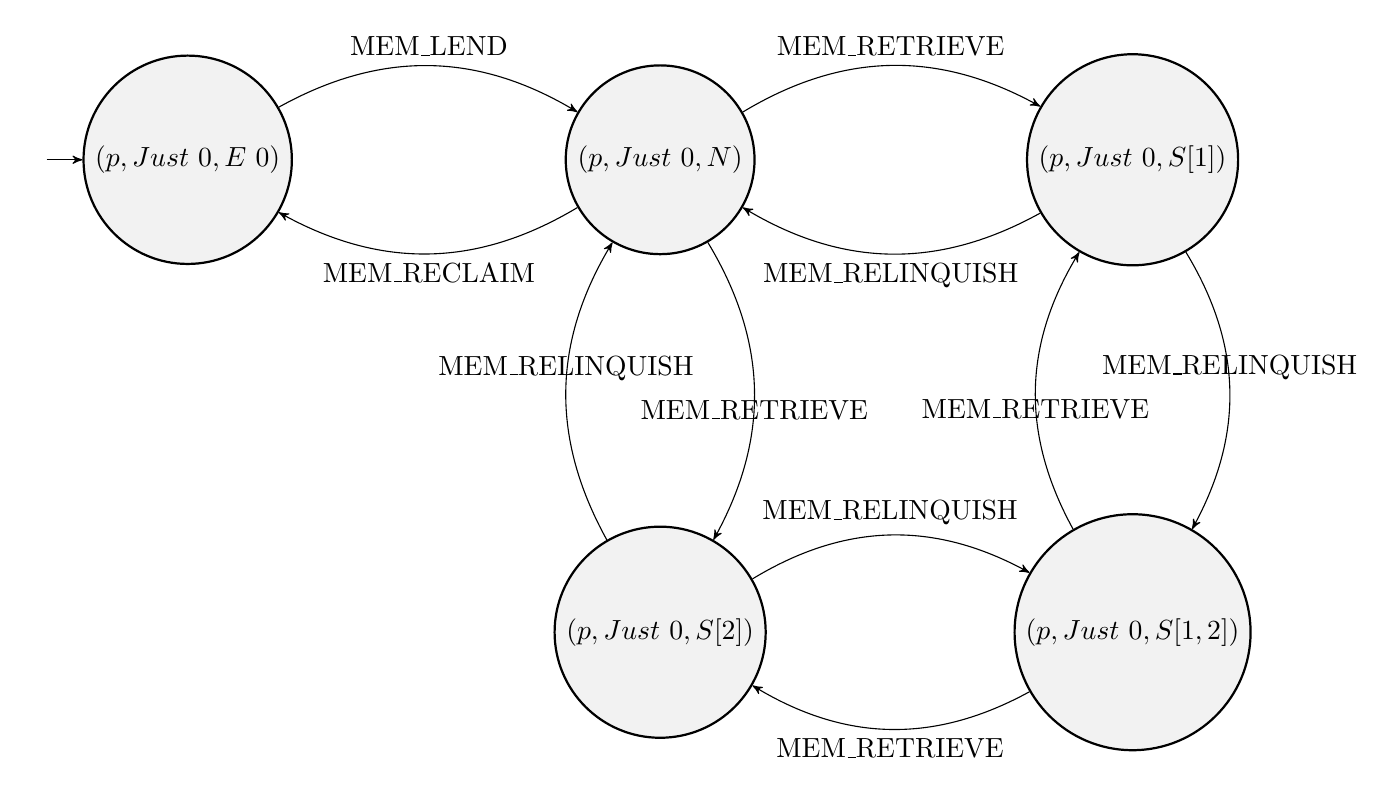
\begin{tikzpicture}
    \node[state, initial, align=center] (q1) {$(p, Just\ 0, E\ 0)$};
    \node[state, right of=q1, align=center] (q2) {$(p, Just\ 0, N)$};
    \node[state, right of=q2, align=center] (q3) {$(p, Just\ 0, S [1])$};
    \node[state, below of=q2, align=center] (q4) {$(p, Just\ 0, S [2])$};
    \node[state, right of=q4, align=center] (q5) {$(p, Just\ 0, S [1,2])$};
    
    \draw   (q1) edge[above, bend left] node{MEM\_LEND} (q2)
            (q2) edge[above, bend left] node{MEM\_RETRIEVE} (q3)
            (q3) edge[below, bend left] node{MEM\_RELINQUISH} (q2)
            (q2) edge[below, bend left] node{MEM\_RETRIEVE} (q4)
            (q4) edge[above, bend left] node{MEM\_RELINQUISH} (q2)
            (q2) edge[below, bend left] node{MEM\_RECLAIM} (q1)
            (q5) edge[below, bend left] node{MEM\_RETRIEVE} (q4)
            (q4) edge[above, bend left] node{MEM\_RELINQUISH} (q5)
            (q5) edge[below, bend left] node{MEM\_RETRIEVE} (q3)
            (q3) edge[above, bend left] node{MEM\_RELINQUISH} (q5);
\end{tikzpicture}
\end{figure}

\clearpage

\begin{lstlisting}[caption={VM 0}]
# save 42
mov R0, addr(p, 0)              # p address
mov R1, 42                      # payload
str R0, R1                      # write payload to p

# mem_lend
# arguments
mov R0, encode_fid(MEM_LEND)    # function id (FFA_MEM_LEND)
mov R1, 8                       # Total length of the  
                                # memory transaction descriptor
# VMID of the Sender 
mov R2, addr(tx, 0)             # TX buffer address                               
mov R3, 0
str R2, R3

# flag
mov R2, addr(tx, 1)             # TX buffer address (offset 1)                               
mov R3, 0                       # not zeroed
str R2, R3

# handle (mbz)
mov R2, addr(tx, 2)             # TX buffer address (offset 2)
mov R3, 0
str R2, R3

# tag (extra information)
mov R2, addr(tx, 3)             # TX buffer address (offset 3)
mov R3, 0
str R2, R3

# access descriptor count
mov R2, addr(tx, 4)             # TX buffer address (offset 4)
mov R3, 2
str R2, R3

# VMID of the first Receiver
mov R2, addr(tx, 5)             # TX buffer address (offset 5)
mov R3, 1
str R2, R3

# base address of the donated page
mov R2, addr(tx, 6)             # TX buffer address (offset 6)
mov R3, addr(p, 0)              # p address
str R2, R3

# VMID of the second Receiver
mov R2, addr(tx, 7)             # TX buffer address (offset 5)
mov R3, 2
str R2, R3

# base address of the donated page
mov R2, addr(tx, 8)             # TX buffer address (offset 6)
mov R3, addr(p, 0)              # p address
str R2, R3

hvc            # [0].pt[p] = (O, NA)
               # [1].pt[p] = (!O, NA)
               # [2].pt[p] = (!O, NA)
               # sss[handler] = 
               # (0, flag, tag, inr (0, [(1, p), (2, p)]), MEM_LEND)

# R2 is populated with the transaction handler at this point
# save it to the discriptor
mov R3, addr(tx, 2)          # TX buffer address (offset 2)
str R3, R2

mov R4, R2                   # save the handler for later

# msg_send to 1
mov R0, encode_fid(MSG_SEND)    # function id (FFA_MSG_SEND)
mov R1, 1                       # VMID of the Receiver
mov R2, 8                       # message length
hvc

# run 1
mov R0, encode_fid(FFA_RUN)
mov R1, 1
hvc

# msg_send to 2
mov R1, 2                       # VMID of the Receiver
mov R2, 8                       # message length
hvc

# run 2
mov R0, encode_fid(FFA_RUN)
mov R1, 2
hvc

# reclaim
mov R0, encode_id(MEM_RECLAIM)
mov R2, R4                       # handler
mov R3, 0                        # flag
hvc            # [0].pt[p] = (O, EA)
               # [1].pt[p] = (!O, NA)
               # [2].pt[p] = (!O, NA)
               # find(sss, handler) = False       
\end{lstlisting}

\begin{lstlisting}[caption={VM 1}]
# retrieve msg length
mov R0, encode_fid(MSG_WAIT)   # function id (FFA_MSG_WAIT)
hvc

# R1 is populated with length of the message at this point

# Copy RX to TX
mov R0, 0             # value to compare with
mov R2, loop          # jump point
mov R3, 1             # step
mov R4, addr(rx, 0)   # RX buffer base address
mov R5, addr(tx, 0)   # TX buffer base address
loop:
sub R1, R1, R3
cmp R1, R0
ldr R6, R4
str R5, R6
add R4, R4, R3
bne R2

mov R0, encode_fid(MEM_RETRIEVE_REQ) # function id (FFA_MEM_RETRIEVE_REQ)
mov R1, 4                            # Total length of the  
                                     # memory transaction descriptor in bytes
# access descriptor count (must be 0 for mem_retrieve)
mov R2, addr(tx, 4)                  # TX buffer address (offset 4)
mov R3, 0
str R2, R3                                    
hvc            # [0].pt[p] = (O, NA)
               # [1].pt[p] = (!O, SA)
               # [2].pt[p] = (!O, NA)
               # sss[handler] = 
               # (0, flag, tag, inr (1, [(1, p), (2, p)]), MEM_LEND)

# save 24
mov R0, addr(p, 0)              # p address
mov R1, 24                      # payload
str R0, R1                      # write payload to p

# handler for relinquishing
mov R0, encode_fid(MEM_RELINQUISH)
mov R1, addr(tx, 2)
ldr R2, R1                      # save the old handler
mov R1, addr(tx, 1)
ldr R3, R1                      # save the old flag
mov R1, addr(tx, 0)             # TX buffer address
str R1, R2                      # handler for a new descriptor
mov R1, addr(tx, 1)
str R1, R3                      # flag for a new descriptor
hvc            # [0].pt[p] = (O, NA)
               # [1].pt[p] = (!O, NA)
               # [2].pt[p] = (!O, NA)
               # sss[handler] = 
               # (0, flag, tag, inr (0, [(1, p), (2, p)]), MEM_LEND)

# yield
mov R0, encode_fid(YIELD)     # function id (FFA_YIELD)
hvc
\end{lstlisting}

\begin{lstlisting}[caption={VM 2}]
# retrieve msg length
mov R0, encode_fid(MSG_WAIT)   # function id (FFA_MSG_WAIT)
hvc

# R1 is populated with length of the message at this point

# Copy RX to TX
mov R0, 0             # value to compare with
mov R2, loop          # jump point
mov R3, 1             # step
mov R4, addr(rx, 0)   # RX buffer base address
mov R5, addr(tx, 0)   # TX buffer base address
loop:
sub R1, R1, R3
cmp R1, R0
ldr R6, R4
str R5, R6
add R4, R4, R3
bne R2

mov R0, encode_fid(MEM_RETRIEVE_REQ) # function id (FFA_MEM_RETRIEVE_REQ)
mov R1, 4                            # Total length of the  
                                     # memory transaction descriptor in bytes
# access descriptor count (must be 0 for mem_retrieve)
mov R2, addr(tx, 4)                  # TX buffer address (offset 4)
mov R3, 0
str R2, R3                                    
hvc            # [0].pt[p] = (O, NA)
               # [1].pt[p] = (!O, NA)
               # [2].pt[p] = (!O, SA)
               # sss[handler] = 
               # (0, flag, tag, inr (1, [(1, p), (2, p)]), MEM_LEND)

# handler for relinquishing
mov R0, encode_fid(MEM_RELINQUISH)
mov R1, addr(tx, 2)
ldr R2, R1                      # save the old handler
mov R1, addr(tx, 1)
ldr R3, R1                      # save the old flag
mov R1, addr(tx, 0)             # TX buffer address
str R1, R2                      # handler for a new descriptor
mov R1, addr(tx, 1)
str R1, R3                      # flag for a new descriptor
hvc            # [0].pt[p] = (O, NA)
               # [1].pt[p] = (!O, NA)
               # [2].pt[p] = (!O, NA)
               # sss[handler] = 
               # (0, flag, tag, inr (0, [(1, p), (2, p)]), MEM_LEND)

# yield
mov R0, encode_fid(YIELD)     # function id (FFA_YIELD)
hvc
\end{lstlisting}

\subsection{Scheduler $\rightarrow$ secondary VM}

Initially, VM 0 has both ownership and exclusive access to page $p$. After a complete lending transaction it loses an access to this page, and passes exclusive access to VM 1. After that, VM 1 relinquish access to the page, and the initial owner reclaims access.

More precisely, VM 0 initiates a memory lending transaction by populating a memory transaction descriptor (within its TX buffer) with receivers' IDs, PIDs, and some auxiliary information. R0 is populated with a function id of FFA\_MEM\_LEND, R1 is populated with a length of a memory descriptor. FFA\_MEM\_LEND returns a handle for this transaction. At this point, VM 0 owns the page but loses access to it. After the transaction initiation, VM 0 populates the memory transaction descriptor with the handle, and sends it via FFA\_MSG\_SEND (perhaps, without endpoint array), and transfers control to VM 1. VM 1 copies the memory transaction descriptor from its RX to TX buffer, and finishes the transaction by calling FFA\_MEM\_RETRIEVE. Now, VM 1 has exclusive access to the page. After that, VM 1 manipulate its newly acquired memory, relinquishes its access to it, and yields control back to VM 0. VM 0 reclaims access to the page.

\begin{figure}[hbt!]
\centering
\begin{sequencediagram}
    \newinst{Hyp}{Hypervisor}
    \newinst[3]{VM0}{VM 0}
    \newinst[3]{VM1}{VM 1}
    
    \begin{call}{VM0}{MEM\_LEND (1)}{Hyp}{SUCCESS}
    \end{call}
    
    \begin{call}{VM0}{MSG\_SEND (1)}{Hyp}{}
    \end{call}
    
    \begin{returnanother}{VM0}{RUN (1)}{Hyp}{}{VM1}
    \end{returnanother}    
    
    \begin{call}{VM1}{MSG\_WAIT}{Hyp}{MSG\_SEND}
    \end{call}
    
    \begin{call}{VM1}{MEM\_RETRIEVE\_REQ}{Hyp}{MEM\_RETRIEVE\_RESP}
    \end{call}
    
    \begin{call}{VM1}{MEM\_RELINQUISH}{Hyp}{SUCCESS}
    \end{call}
    
    \begin{returnanother}{VM1}{YIELD}{Hyp}{}{VM0}
    \end{returnanother}  
    
    \begin{call}{VM0}{MEM\_RECLAIM}{Hyp}{SUCCESS}
    \end{call}  
       
\end{sequencediagram}

\end{figure}

\begin{figure}[hbt!]
\centering
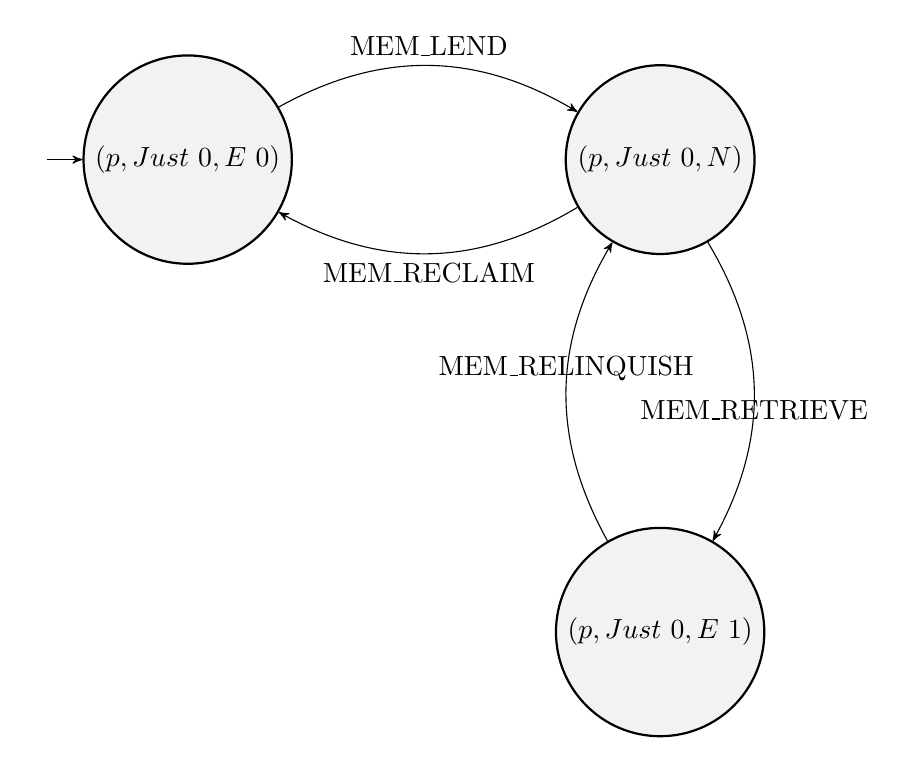
\begin{tikzpicture}
    \node[state, initial, align=center] (q1) {$(p, Just\ 0, E\ 0)$};
    \node[state, right of=q1, align=center] (q2) {$(p, Just\ 0, N)$};
    \node[state, below of=q2, align=center] (q3) {$(p, Just\ 0, E\ 1)$};
    
    \draw   (q1) edge[above, bend left] node{MEM\_LEND} (q2)
            (q2) edge[below, bend left] node{MEM\_RETRIEVE} (q3)
            (q3) edge[above, bend left] node{MEM\_RELINQUISH} (q2)
            (q2) edge[below, bend left] node{MEM\_RECLAIM} (q1);
\end{tikzpicture}
\end{figure}

\clearpage

\begin{lstlisting}[caption={VM 0}]
# save 42
mov R0, addr(p, 0)              # p address
mov R1, 42                      # payload
str R0, R1                      # write payload to p

# mem_lend
# arguments
mov R0, encode_fid(MEM_LEND)    # function id (FFA_MEM_LEND)
mov R1, 8                       # Total length of the  
                                # memory transaction descriptor
# VMID of the Sender 
mov R2, addr(tx, 0)             # TX buffer address                               
mov R3, 0
str R2, R3

# flag
mov R2, addr(tx, 1)             # TX buffer address (offset 1)                               
mov R3, 0                       # not zeroed
str R2, R3

# handle (mbz)
mov R2, addr(tx, 2)             # TX buffer address (offset 2)
mov R3, 0
str R2, R3

# tag (extra information)
mov R2, addr(tx, 3)             # TX buffer address (offset 3)
mov R3, 0
str R2, R3

# access descriptor count
mov R2, addr(tx, 4)             # TX buffer address (offset 4)
mov R3, 1
str R2, R3

# VMID of the first Receiver
mov R2, addr(tx, 5)             # TX buffer address (offset 5)
mov R3, 1
str R2, R3

# base address of the donated page
mov R2, addr(tx, 6)             # TX buffer address (offset 6)
mov R3, addr(p, 0)              # p address
str R2, R3

hvc            # [0].pt[p] = (O, NA)
               # [1].pt[p] = (!O, NA)
               # sss[handler] = 
               # (0, flag, tag, inl (1, p), MEM_LEND)

# R2 is populated with the transaction handler at this point
# save it to the discriptor
mov R3, addr(tx, 2)          # TX buffer address (offset 2)
str R3, R2

mov R4, R2                   # save the handler for later

# msg_send to 1
mov R0, encode_fid(MSG_SEND)    # function id (FFA_MSG_SEND)
mov R1, 1                       # VMID of the Receiver
mov R2, 8                       # message length
hvc

# run 1
mov R0, encode_fid(FFA_RUN)
mov R1, 1
hvc

# reclaim
mov R0, encode_id(MEM_RECLAIM)
mov R2, R4                       # handler
mov R3, 0                        # flag
hvc            # [0].pt[p] = (O, EA)
               # [1].pt[p] = (!O, NA)
               # find(sss, handler) = False       
\end{lstlisting}

\begin{lstlisting}[caption={VM 1}]
# retrieve msg length
mov R0, encode_fid(MSG_WAIT)   # function id (FFA_MSG_WAIT)
hvc

# R1 is populated with length of the message at this point

# Copy RX to TX
mov R0, 0             # value to compare with
mov R2, loop          # jump point
mov R3, 1             # step
mov R4, addr(rx, 0)   # RX buffer base address
mov R5, addr(tx, 0)   # TX buffer base address
loop:
sub R1, R1, R3
cmp R1, R0
ldr R6, R4
str R5, R6
add R4, R4, R3
bne R2

mov R0, encode_fid(MEM_RETRIEVE_REQ) # function id (FFA_MEM_RETRIEVE_REQ)
mov R1, 4                            # Total length of the  
                                     # memory transaction descriptor in bytes
# access descriptor count (must be 0 for mem_retrieve)
mov R2, addr(tx, 4)                  # TX buffer address (offset 4)
mov R3, 0
str R2, R3                                    
hvc            # [0].pt[p] = (O, NA)
               # [1].pt[p] = (!O, EA)
               # sss[handler] = 
               # (0, flag, tag, inl (1, p), MEM_LEND)

# save 24
mov R0, addr(p, 0)              # p address
mov R1, 24                      # payload
str R0, R1                      # write payload to p

# handler for relinquishing
mov R0, encode_fid(MEM_RELINQUISH)
mov R1, addr(tx, 2)
ldr R2, R1                      # save the old handler
mov R1, addr(tx, 1)
ldr R3, R1                      # save the old flag
mov R1, addr(tx, 0)             # TX buffer address
str R1, R2                      # handler for a new descriptor
mov R1, addr(tx, 1)
str R1, R3                      # flag for a new descriptor
hvc            # [0].pt[p] = (O, NA)
               # [1].pt[p] = (!O, NA)
               # sss[handler] = 
               # (0, flag, tag, inl (1, p), MEM_LEND)

# yield
mov R0, encode_fid(YIELD)     # function id (FFA_YIELD)
hvc
\end{lstlisting}

\subsection{Secondary VM $\rightarrow$ secondary VMs}

Initially, VM 1 has both ownership and exclusive access to page $p$. After a complete lending transaction it loses an access to this page, and passes shared access to VM 2 and VM 3. In case, it would transfer access only to a single VM, it'll grant this VM with exclusive access. After that, the initial owner reclaims access.

More precisely, VM 0 gives control to VM 1, which in turn initiates a memory lending transaction by populating a memory transaction descriptor (within its TX buffer) with receivers' IDs, PIDs, and some auxiliary information. R0 is populated with a function id of FFA\_MEM\_LEND, R1 is populated with a length of a memory descriptor. FFA\_MEM\_LEND returns a handle for this transaction. At this point, VM 1 owns the page but loses access to it. After the transaction initiation, VM 1 populates the memory transaction descriptor with the handle, and sends it via FFA\_MSG\_SEND (perhaps, without endpoint array), and yields control to VM 0. VM 0 transfers control to VM 2. VM 2 copies the memory transaction descriptor from RX to TX buffer, and finishes the transaction by calling FFA\_MEM\_RETRIEVE. Now, VM 2 has shared access to the page. After that, VM 2 manipulates its newly acquired memory, relinquishes its access to it, and yields control back to VM 0. VM 0 transfers control to VM 3, which does the same sequence of operations as VM 2 did. Now, VM 0 can transfer control to VM 1, which reclaims access to the page.

\begin{figure}[hbt!]
\centering
\begin{sequencediagram}
    \newinst{Hyp}{Hypervisor}
    \newinst[2]{VM0}{VM 0}
    \newinst[2]{VM1}{VM 1}
    \newinst[2]{VM2}{VM 2}
    \newinst[2]{VM3}{VM 3}
    
    \begin{returnanother}{VM0}{RUN (1)}{Hyp}{}{VM1}
    \end{returnanother}
    
    \begin{call}{VM1}{MEM\_LEND (2,3)}{Hyp}{SUCCESS}
    \end{call}
    
    \begin{returnanother}{VM1}{MSG\_SEND (2)}{Hyp}{}{VM0}
    \end{returnanother}
    
    \begin{returnanother}{VM0}{RUN (2)}{Hyp}{}{VM2}
    \end{returnanother}    
    
    \begin{call}{VM2}{MSG\_WAIT}{Hyp}{MSG\_SEND}
    \end{call}
    
    \begin{call}{VM2}{MEM\_RETRIEVE\_REQ}{Hyp}{MEM\_RETRIEVE\_RESP}
    \end{call}
    
    \begin{call}{VM2}{MEM\_RELINQUISH}{Hyp}{SUCCESS}
    \end{call}
    
    \begin{returnanother}{VM2}{YIELD}{Hyp}{}{VM0}
    \end{returnanother}
    
    \begin{returnanother}{VM0}{RUN (3)}{Hyp}{}{VM3}
    \end{returnanother}    
    
    \begin{call}{VM3}{MSG\_WAIT}{Hyp}{MSG\_SEND}
    \end{call}
    
    \begin{call}{VM3}{MEM\_RETRIEVE\_REQ}{Hyp}{MEM\_RETRIEVE\_RESP}
    \end{call}
    
    \begin{call}{VM3}{MEM\_RELINQUISH}{Hyp}{SUCCESS}
    \end{call}
    
    \begin{returnanother}{VM3}{YIELD}{Hyp}{}{VM0}
    \end{returnanother} 
    
    \begin{returnanother}{VM0}{RUN (1)}{Hyp}{}{VM1}
    \end{returnanother}  
    
    \begin{call}{VM1}{MEM\_RECLAIM}{Hyp}{SUCCESS}
    \end{call}  
    
    \begin{returnanother}{VM1}{YIELD}{Hyp}{}{VM0}
    \end{returnanother} 
       
\end{sequencediagram}
\end{figure}

\begin{figure}[hbt!]
\flushright
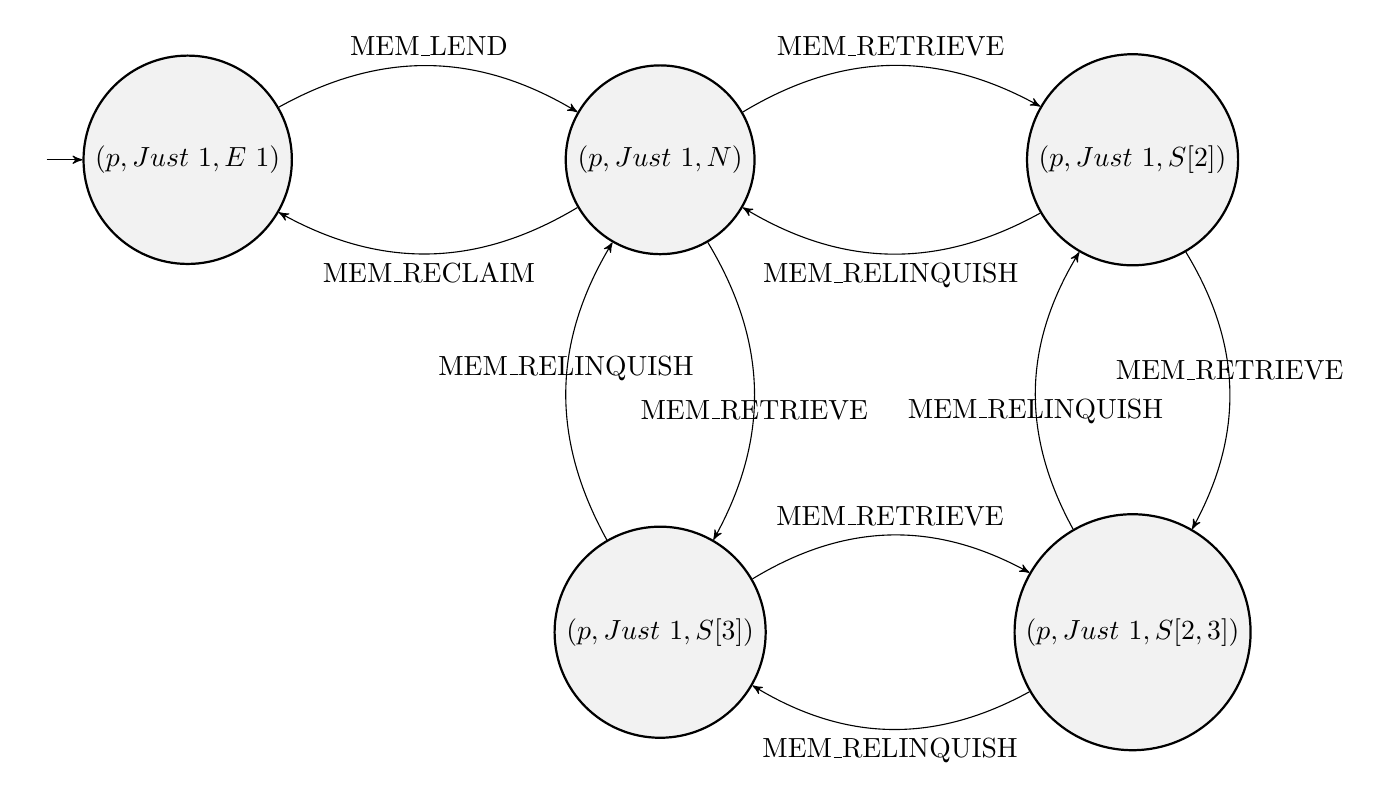
\begin{tikzpicture}
    \node[state, initial, align=center] (q1) {$(p, Just\ 1, E\ 1)$};
    \node[state, right of=q1, align=center] (q2) {$(p, Just\ 1, N)$};
    \node[state, right of=q2, align=center] (q3) {$(p, Just\ 1, S [2])$};
    \node[state, below of=q2, align=center] (q4) {$(p, Just\ 1, S [3])$};
    \node[state, right of=q4, align=center] (q5) {$(p, Just\ 1, S [2,3])$};
    
    \draw   (q1) edge[above, bend left] node{MEM\_LEND} (q2)
            (q2) edge[above, bend left] node{MEM\_RETRIEVE} (q3)
            (q3) edge[below, bend left] node{MEM\_RELINQUISH} (q2)
            (q2) edge[below, bend left] node{MEM\_RETRIEVE} (q4)
            (q4) edge[above, bend left] node{MEM\_RELINQUISH} (q2)
            (q2) edge[below, bend left] node{MEM\_RECLAIM} (q1)   
            (q3) edge[above, bend left] node{MEM\_RETRIEVE} (q5)
            (q5) edge[below, bend left] node{MEM\_RELINQUISH} (q3)
            (q4) edge[above, bend left] node{MEM\_RETRIEVE} (q5)
            (q5) edge[below, bend left] node{MEM\_RELINQUISH} (q4);
\end{tikzpicture}
\end{figure}

\clearpage

\begin{lstlisting}[caption={VM 0}]
# run 1 (to lend)
mov R0, encode_fid(FFA_RUN) # function id (FFA_RUN)
mov R1, 1                   # callee VMID
hvc

# run 2 (to retrieve and relinquish)
mov R0, encode_fid(FFA_RUN) # function id (FFA_RUN)
mov R1, 3                   # callee VMID
hvc

# run 1 (to send a message to VM 3)
mov R0, encode_fid(FFA_RUN) # function id (FFA_RUN)
mov R1, 1                   # callee VMID
hvc

# run 3 (to retrieve and relinquish)
mov R0, encode_fid(FFA_RUN) # function id (FFA_RUN)
mov R1, 3                   # callee VMID
hvc

# run 1 (to reclaim)
mov R0, encode_fid(FFA_RUN) # function id (FFA_RUN)
mov R1, 1                   # callee VMID
hvc
\end{lstlisting}

\begin{lstlisting}[caption={VM 1}]
# save 42
mov R0, addr(p, 0)              # p address
mov R1, 42                      # payload
str R0, R1                      # write payload to p

# mem_lend
# arguments
mov R0, encode_fid(MEM_LEND)    # function id (FFA_MEM_LEND)
mov R1, 8                       # Total length of the  
                                # memory transaction descriptor
# VMID of the sender 
mov R2, addr(tx, 0)             # TX buffer address                               
mov R3, 1
str R2, R3

# flag
mov R2, addr(tx, 1)             # TX buffer address (offset 1)                               
mov R3, 0                       # not zeroed
str R2, R3

# handle (mbz)
mov R2, addr(tx, 2)             # TX buffer address (offset 2)
mov R3, 0
str R2, R3

# tag (extra information)
mov R2, addr(tx, 3)             # TX buffer address (offset 3)
mov R3, 0
str R2, R3

# access descriptor count
mov R2, addr(tx, 4)             # TX buffer address (offset 4)
mov R3, 2
str R2, R3

# VMID of the first Receiver
mov R2, addr(tx, 5)             # TX buffer address (offset 5)
mov R3, 2
str R2, R3

# base address of the donated page
mov R2, addr(tx, 6)             # TX buffer address (offset 6)
mov R3, addr(p, 0)              # p address
str R2, R3

# VMID of the second Receiver
mov R2, addr(tx, 7)             # TX buffer address (offset 5)
mov R3, 3
str R2, R3

# base address of the donated page
mov R2, addr(tx, 8)             # TX buffer address (offset 6)
mov R3, addr(p, 0)              # p address
str R2, R3

hvc            # [0].pt[p] = (!O, NA)
               # [1].pt[p] = (O, NA)
               # [2].pt[p] = (!O, NA)
               # [3].pt[p] = (!O, NA)
               # sss[handler] = 
               # (1, flag, tag, inr (0, [(2, p), (3, p)]), MEM_LEND)

# R2 is populated with the transaction handler at this point
# save it to the discriptor
mov R3, addr(tx, 2)          # TX buffer address (offset 2)
str R3, R2

mov R4, R2                   # save the handler for later

# msg_send to 2
mov R0, encode_fid(MSG_SEND)    # function id (FFA_MSG_SEND)
mov R1, 2                       # VMID of the Receiver
mov R2, 8                       # message length
hvc

# msg_send to 3
mov R1, 3                       # VMID of the Receiver
mov R2, 8                       # message length
hvc

# reclaim
mov R0, encode_id(MEM_RECLAIM)
mov R2, R4                       # handler
mov R3, 0                        # flag
hvc            # [0].pt[p] = (!O, NA)
               # [1].pt[p] = (O, EA)
               # [2].pt[p] = (!O, NA)
               # [3].pt[p] = (!O, NA)
               # find(sss, handler) = False  
               
# yield
mov R0, encode_fid(YIELD)     # function id (FFA_YIELD)
hvc     
\end{lstlisting}

\begin{lstlisting}[caption={VM 2}]
# retrieve msg length
mov R0, encode_fid(MSG_WAIT)   # function id (FFA_MSG_WAIT)
hvc

# R1 is populated with length of the message at this point

# Copy RX to TX
mov R0, 0             # value to compare with
mov R2, loop          # jump point
mov R3, 1             # step
mov R4, addr(rx, 0)   # RX buffer base address
mov R5, addr(tx, 0)   # TX buffer base address
loop:
sub R1, R1, R3
cmp R1, R0
ldr R6, R4
str R5, R6
add R4, R4, R3
bne R2

mov R0, encode_fid(MEM_RETRIEVE_REQ) # function id (FFA_MEM_RETRIEVE_REQ)
mov R1, 4                            # Total length of the  
                                     # memory transaction descriptor in bytes
# access descriptor count (must be 0 for mem_retrieve)
mov R2, addr(tx, 4)                  # TX buffer address (offset 4)
mov R3, 0
str R2, R3                                    
hvc            # [0].pt[p] = (!O, NA)
               # [1].pt[p] = (O, NA)
               # [2].pt[p] = (!O, SA)
               # [3].pt[p] = (!O, NA)
               # sss[handler] = 
               # (1, flag, tag, inr (1, [(2, p), (3, p)]), MEM_LEND)

# save 24
mov R0, addr(p, 0)              # p address
mov R1, 24                      # payload
str R0, R1                      # write payload to p

# handler for relinquishing
mov R0, encode_fid(MEM_RELINQUISH)
mov R1, addr(tx, 2)
ldr R2, R1                      # save the old handler
mov R1, addr(tx, 1)
ldr R3, R1                      # save the old flag
mov R1, addr(tx, 0)             # TX buffer address
str R1, R2                      # handler for a new descriptor
mov R1, addr(tx, 1)
str R1, R3                      # flag for a new descriptor
hvc            # [0].pt[p] = (!O, NA)
               # [1].pt[p] = (O, NA)
               # [2].pt[p] = (!O, NA)
               # [3].pt[p] = (!O, NA)
               # sss[handler] = 
               # (1, flag, tag, inr (0, [(2, p), (3, p)]), MEM_LEND)

# yield
mov R0, encode_fid(YIELD)     # function id (FFA_YIELD)
hvc
\end{lstlisting}

\begin{lstlisting}[caption={VM 3}]
# retrieve msg length
mov R0, encode_fid(MSG_WAIT)   # function id (FFA_MSG_WAIT)
hvc

# R1 is populated with length of the message at this point

# Copy RX to TX
mov R0, 0             # value to compare with
mov R2, loop          # jump point
mov R3, 1             # step
mov R4, addr(rx, 0)   # RX buffer base address
mov R5, addr(tx, 0)   # TX buffer base address
loop:
sub R1, R1, R3
cmp R1, R0
ldr R6, R4
str R5, R6
add R4, R4, R3
bne R2

mov R0, encode_fid(MEM_RETRIEVE_REQ) # function id (FFA_MEM_RETRIEVE_REQ)
mov R1, 4                            # Total length of the  
                                     # memory transaction descriptor in bytes
# access descriptor count (must be 0 for mem_retrieve)
mov R2, addr(tx, 4)                  # TX buffer address (offset 4)
mov R3, 0
str R2, R3                                    
hvc            # [0].pt[p] = (!O, NA)
               # [1].pt[p] = (O, NA)
               # [2].pt[p] = (!O, NA)
               # [3].pt[p] = (!O, SA)
               # sss[handler] = 
               # (1, flag, tag, inr (1, [(2, p), (3, p)]), MEM_LEND)

# handler for relinquishing
mov R0, encode_fid(MEM_RELINQUISH)
mov R1, addr(tx, 2)
ldr R2, R1                      # save the old handler
mov R1, addr(tx, 1)
ldr R3, R1                      # save the old flag
mov R1, addr(tx, 0)             # TX buffer address
str R1, R2                      # handler for a new descriptor
mov R1, addr(tx, 1)
str R1, R3                      # flag for a new descriptor
hvc            # [0].pt[p] = (!O, NA)
               # [1].pt[p] = (O, NA)
               # [2].pt[p] = (!O, NA)
               # [3].pt[p] = (!O, NA)
               # sss[handler] = 
               # (1, flag, tag, inr (0, [(2, p), (3, p)]), MEM_LEND)

# yield
mov R0, encode_fid(YIELD)     # function id (FFA_YIELD)
hvc
\end{lstlisting}

\section{Memory sharing}

\subsection{Scheduler $\rightarrow$ secondary VMs}

\begin{figure}[hbt!]
\centering
\begin{sequencediagram}
    \newinst{Hyp}{Hypervisor}
    \newinst[3]{VM0}{VM 0}
    \newinst[3]{VM1}{VM 1}
    \newinst[3]{VM2}{VM 2}
    
    \begin{call}{VM0}{MEM\_SHARE (1,2)}{Hyp}{SUCCESS}
    \end{call}
    
    \begin{call}{VM0}{MSG\_SEND (1)}{Hyp}{}
    \end{call}
    
    \begin{returnanother}{VM0}{RUN (1)}{Hyp}{}{VM1}
    \end{returnanother}
    
    \begin{call}{VM1}{MEM\_RETRIEVE\_REQ}{Hyp}{MEM\_RETRIEVE\_RESP}
    \end{call}
    
    \begin{call}{VM1}{MEM\_RELINQUISH}{Hyp}{SUCCESS}
    \end{call}
    
    \begin{returnanother}{VM1}{YIELD}{Hyp}{}{VM0}
    \end{returnanother}
    
    \begin{call}{VM0}{MSG\_SEND (2)}{Hyp}{}
    \end{call}
    
    \begin{returnanother}{VM0}{RUN (2)}{Hyp}{}{VM2}
    \end{returnanother}
    
    \begin{call}{VM2}{MEM\_RETRIEVE\_REQ}{Hyp}{MEM\_RETRIEVE\_RESP}
    \end{call}
    
    \begin{call}{VM2}{MEM\_RELINQUISH}{Hyp}{SUCCESS}
    \end{call}
    
    \begin{returnanother}{VM2}{YIELD}{Hyp}{}{VM0}
    \end{returnanother}
    
    \begin{call}{VM0}{MEM\_RECLAIM}{Hyp}{SUCCESS}
    \end{call}  
       
\end{sequencediagram}
\end{figure}

\begin{figure}[hbt!]
\centering
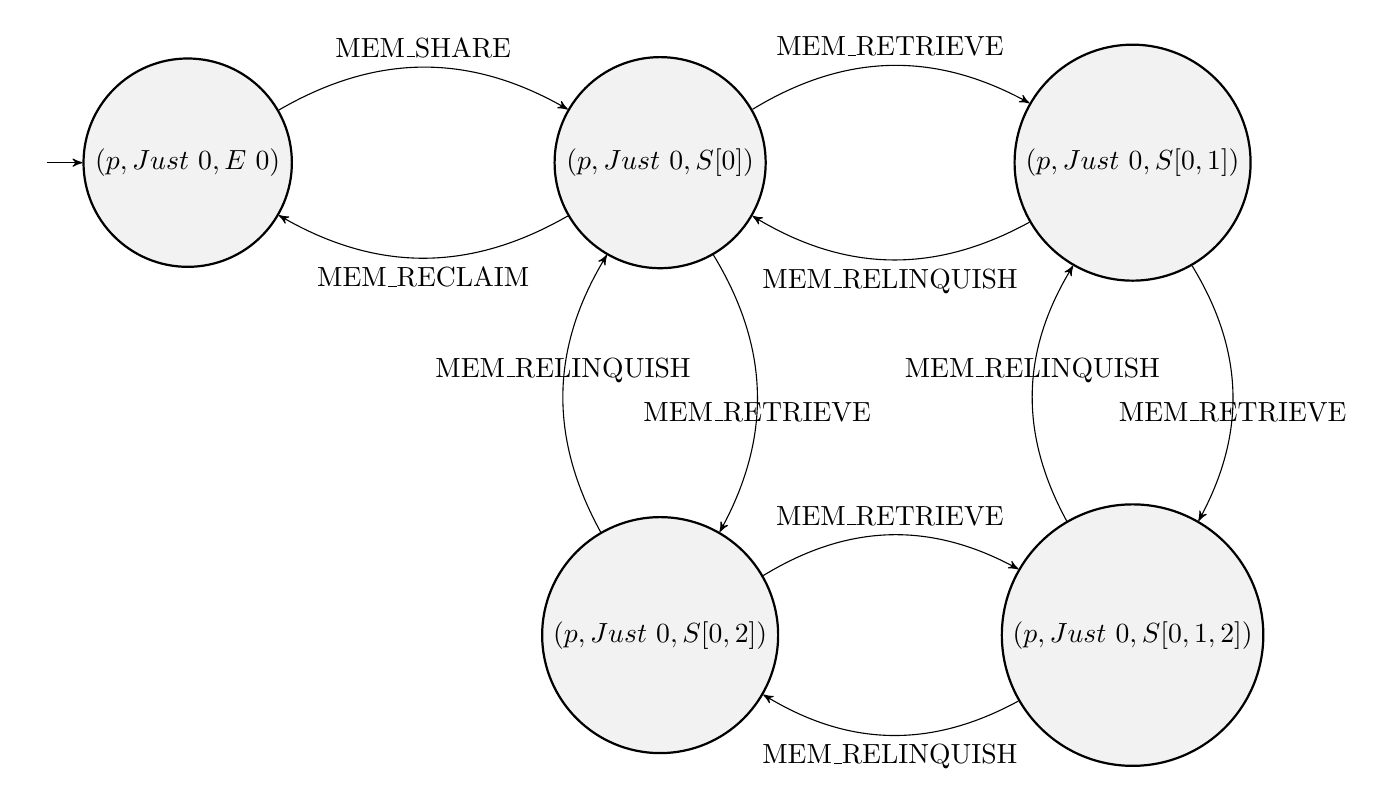
\begin{tikzpicture}
    \node[state, initial, align=center] (q1) {$(p, Just\ 0, E\ 0)$};
    \node[state, right of=q1, align=center] (q2) {$(p, Just\ 0, S [0])$};
    \node[state, right of=q2, align=center] (q3) {$(p, Just\ 0, S [0, 1])$};
    \node[state, below of=q2, align=center] (q4) {$(p, Just\ 0, S [0, 2])$};
    \node[state, right of=q4, align=center] (q5) {$(p, Just\ 0, S [0, 1, 2])$};
    
    \draw   (q1) edge[above, bend left] node{MEM\_SHARE} (q2)
            (q2) edge[above, bend left] node{MEM\_RETRIEVE} (q3)
            (q3) edge[below, bend left] node{MEM\_RELINQUISH} (q2)
            (q2) edge[below, bend left] node{MEM\_RETRIEVE} (q4)
            (q4) edge[above, bend left] node{MEM\_RELINQUISH} (q2)
            (q2) edge[below, bend left] node{MEM\_RECLAIM} (q1)           
            (q3) edge[below, bend left] node{MEM\_RETRIEVE} (q5)
            (q5) edge[above, bend left] node{MEM\_RELINQUISH} (q3)
            (q4) edge[above, bend left] node{MEM\_RETRIEVE} (q5)
            (q5) edge[below, bend left] node{MEM\_RELINQUISH} (q4);
\end{tikzpicture}
\end{figure}

\clearpage

\begin{lstlisting}[caption={VM 0}]
# save 42
mov R0, addr(p, 0)              # p address
mov R1, 42                      # payload
str R0, R1                      # write payload to p

# mem_lend
# arguments
mov R0, encode_fid(MEM_SHARE)   # function id (FFA_MEM_SHARE)
mov R1, 8                       # Total length of the  
                                # memory transaction descriptor
# VMID of the Sender 
mov R2, addr(tx, 0)             # TX buffer address                               
mov R3, 0
str R2, R3

# flag
mov R2, addr(tx, 1)             # TX buffer address (offset 1)                               
mov R3, 0                       # not zeroed
str R2, R3

# handle (mbz)
mov R2, addr(tx, 2)             # TX buffer address (offset 2)
mov R3, 0
str R2, R3

# tag (extra information)
mov R2, addr(tx, 3)             # TX buffer address (offset 3)
mov R3, 0
str R2, R3

# access descriptor count
mov R2, addr(tx, 4)             # TX buffer address (offset 4)
mov R3, 2
str R2, R3

# VMID of the first Receiver
mov R2, addr(tx, 5)             # TX buffer address (offset 5)
mov R3, 1
str R2, R3

# base address of the donated page
mov R2, addr(tx, 6)             # TX buffer address (offset 6)
mov R3, addr(p, 0)              # p address
str R2, R3

# VMID of the second Receiver
mov R2, addr(tx, 7)             # TX buffer address (offset 5)
mov R3, 2
str R2, R3

# base address of the donated page
mov R2, addr(tx, 8)             # TX buffer address (offset 6)
mov R3, addr(p, 0)              # p address
str R2, R3

hvc            # [0].pt[p] = (O, SA)
               # [1].pt[p] = (!O, NA)
               # [2].pt[p] = (!O, NA)
               # sss[handler] = 
               # (0, flag, tag, inr (0, [(1, p), (2, p)]), MEM_SHARE)

# R2 is populated with the transaction handler at this point
# save it to the discriptor
mov R3, addr(tx, 2)          # TX buffer address (offset 2)
str R3, R2

mov R4, R2                   # save the handler for later

# msg_send to 1
mov R0, encode_fid(MSG_SEND)    # function id (FFA_MSG_SEND)
mov R1, 1                       # VMID of the Receiver
mov R2, 8                       # message length
hvc

# run 1
mov R0, encode_fid(FFA_RUN)
mov R1, 1
hvc

# msg_send to 2
mov R1, 2                       # VMID of the Receiver
mov R2, 8                       # message length
hvc

# run 2
mov R0, encode_fid(FFA_RUN)
mov R1, 2
hvc

# reclaim
mov R0, encode_id(MEM_RECLAIM)
mov R2, R4                       # handler
mov R3, 0                        # flag
hvc            # [0].pt[p] = (O, EA)
               # [1].pt[p] = (!O, NA)
               # [2].pt[p] = (!O, NA)
               # find(sss, handler) = False       
\end{lstlisting}

\begin{lstlisting}[caption={VM 1}]
# retrieve msg length
mov R0, encode_fid(MSG_WAIT)   # function id (FFA_MSG_WAIT)
hvc

# R1 is populated with length of the message at this point

# Copy RX to TX
mov R0, 0             # value to compare with
mov R2, loop          # jump point
mov R3, 1             # step
mov R4, addr(rx, 0)   # RX buffer base address
mov R5, addr(tx, 0)   # TX buffer base address
loop:
sub R1, R1, R3
cmp R1, R0
ldr R6, R4
str R5, R6
add R4, R4, R3
bne R2

mov R0, encode_fid(MEM_RETRIEVE_REQ) # function id (FFA_MEM_RETRIEVE_REQ)
mov R1, 4                            # Total length of the  
                                     # memory transaction descriptor in bytes
# access descriptor count (must be 0 for mem_retrieve)
mov R2, addr(tx, 4)                  # TX buffer address (offset 4)
mov R3, 0
str R2, R3                                    
hvc            # [0].pt[p] = (O, SA)
               # [1].pt[p] = (!O, SA)
               # [2].pt[p] = (!O, NA)
               # sss[handler] = 
               # (0, flag, tag, inr (1, [(1, p), (2, p)]), MEM_SHARE)

# save 24
mov R0, addr(p, 0)              # p address
mov R1, 24                      # payload
str R0, R1                      # write payload to p

# handler for relinquishing
mov R0, encode_fid(MEM_RELINQUISH)
mov R1, addr(tx, 2)
ldr R2, R1                      # save the old handler
mov R1, addr(tx, 1)
ldr R3, R1                      # save the old flag
mov R1, addr(tx, 0)             # TX buffer address
str R1, R2                      # handler for a new descriptor
mov R1, addr(tx, 1)
str R1, R3                      # flag for a new descriptor
hvc            # [0].pt[p] = (O, SA)
               # [1].pt[p] = (!O, NA)
               # [2].pt[p] = (!O, NA)
               # sss[handler] = 
               # (0, flag, tag, inr (0, [(1, p), (2, p)]), MEM_SHARE)

# yield
mov R0, encode_fid(YIELD)     # function id (FFA_YIELD)
hvc
\end{lstlisting}

\begin{lstlisting}[caption={VM 2}]
# retrieve msg length
mov R0, encode_fid(MSG_WAIT)   # function id (FFA_MSG_WAIT)
hvc

# R1 is populated with length of the message at this point

# Copy RX to TX
mov R0, 0             # value to compare with
mov R2, loop          # jump point
mov R3, 1             # step
mov R4, addr(rx, 0)   # RX buffer base address
mov R5, addr(tx, 0)   # TX buffer base address
loop:
sub R1, R1, R3
cmp R1, R0
ldr R6, R4
str R5, R6
add R4, R4, R3
bne R2

mov R0, encode_fid(MEM_RETRIEVE_REQ) # function id (FFA_MEM_RETRIEVE_REQ)
mov R1, 4                            # Total length of the  
                                     # memory transaction descriptor in bytes
# access descriptor count (must be 0 for mem_retrieve)
mov R2, addr(tx, 4)                  # TX buffer address (offset 4)
mov R3, 0
str R2, R3                                    
hvc            # [0].pt[p] = (O, SA)
               # [1].pt[p] = (!O, NA)
               # [2].pt[p] = (!O, SA)
               # sss[handler] = 
               # (0, flag, tag, inr (1, [(1, p), (2, p)]), MEM_SHARE)

# handler for relinquishing
mov R0, encode_fid(MEM_RELINQUISH)
mov R1, addr(tx, 2)
ldr R2, R1                      # save the old handler
mov R1, addr(tx, 1)
ldr R3, R1                      # save the old flag
mov R1, addr(tx, 0)             # TX buffer address
str R1, R2                      # handler for a new descriptor
mov R1, addr(tx, 1)
str R1, R3                      # flag for a new descriptor
hvc            # [0].pt[p] = (O, SA)
               # [1].pt[p] = (!O, NA)
               # [2].pt[p] = (!O, NA)
               # sss[handler] = 
               # (0, flag, tag, inr (0, [(1, p), (2, p)]), MEM_SHARE)

# yield
mov R0, encode_fid(YIELD)     # function id (FFA_YIELD)
hvc
\end{lstlisting}

\subsection{Secondary VM $\rightarrow$ secondary VMs}

\begin{figure}[hbt!]
\centering
\begin{sequencediagram}
    \newinst{Hyp}{Hypervisor}
    \newinst[2]{VM0}{VM 0}
    \newinst[2]{VM1}{VM 1}
    \newinst[2]{VM2}{VM 2}
    \newinst[2]{VM3}{VM 3}

    \begin{returnanother}{VM0}{RUN (1)}{Hyp}{}{VM1}
    \end{returnanother}
    
    \begin{call}{VM1}{MEM\_SHARE (2,3)}{Hyp}{SUCCESS}
    \end{call}
    
    \begin{returnanother}{VM1}{MSG\_SEND (2)}{Hyp}{}{VM0}
    \end{returnanother}
    
    \begin{returnanother}{VM0}{RUN (2)}{Hyp}{}{VM2}
    \end{returnanother}
    
    \begin{call}{VM2}{MSG\_WAIT}{Hyp}{MSG\_SEND}
    \end{call}
    
    \begin{call}{VM2}{MEM\_RETRIEVE\_REQ}{Hyp}{MEM\_RETRIEVE\_RESP}
    \end{call}
    
    \begin{call}{VM2}{MEM\_RELINQUISH}{Hyp}{SUCCESS}
    \end{call}
    
    \begin{returnanother}{VM2}{YIELD}{Hyp}{}{VM0}
    \end{returnanother}   
    
    \begin{returnanother}{VM0}{RUN (1)}{Hyp}{}{VM1}
    \end{returnanother}
    
    \begin{returnanother}{VM1}{MSG\_SEND (3)}{Hyp}{}{VM0}
    \end{returnanother}
    
    \begin{returnanother}{VM0}{RUN (3)}{Hyp}{}{VM3}
    \end{returnanother}
    
    \begin{call}{VM3}{MSG\_WAIT}{Hyp}{MSG\_SEND}
    \end{call}
    
    \begin{call}{VM3}{MEM\_RETRIEVE\_REQ}{Hyp}{MEM\_RETRIEVE\_RESP}
    \end{call}
    
    \begin{call}{VM3}{MEM\_RELINQUISH}{Hyp}{SUCCESS}
    \end{call}
    
    \begin{returnanother}{VM3}{YIELD}{Hyp}{}{VM0}
    \end{returnanother}   
    
    \begin{returnanother}{VM0}{RUN (1)}{Hyp}{}{VM1}
    \end{returnanother}    
    
    \begin{call}{VM1}{MEM\_RECLAIM}{Hyp}{SUCCESS}
    \end{call}  
    
    \begin{returnanother}{VM1}{YIELD}{Hyp}{}{VM0}
    \end{returnanother}  
       
\end{sequencediagram}
\end{figure}

\begin{figure}[hbt!]
\centering
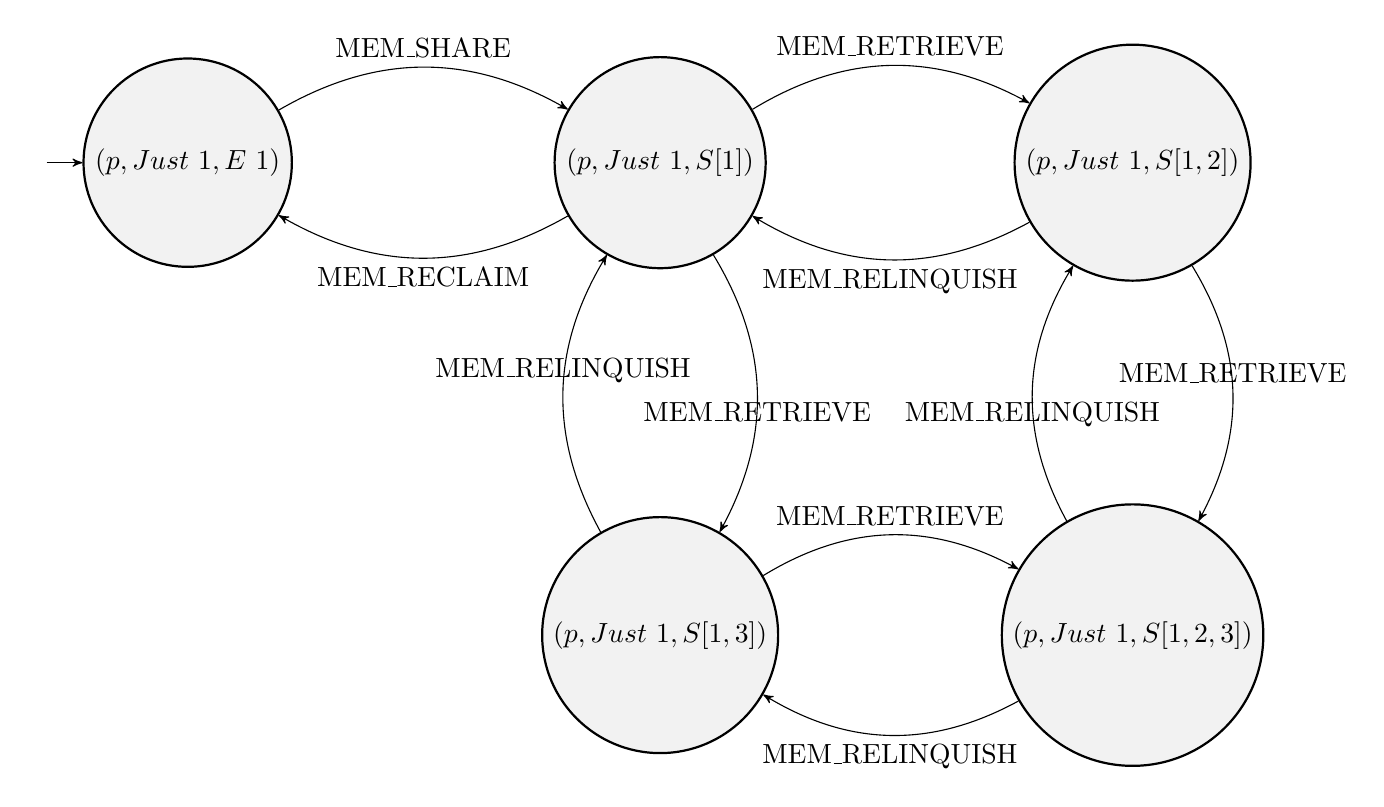
\begin{tikzpicture}
    \node[state, initial, align=center] (q1) {$(p, Just\ 1, E\ 1)$};
    \node[state, right of=q1, align=center] (q2) {$(p, Just\ 1, S [1])$};
    \node[state, right of=q2, align=center] (q3) {$(p, Just\ 1, S [1,2])$};
    \node[state, below of=q2, align=center] (q4) {$(p, Just\ 1, S [1,3])$};
    \node[state, right of=q4, align=center] (q5) {$(p, Just\ 1, S [1,2,3])$};
    
    \draw   (q1) edge[above, bend left] node{MEM\_SHARE} (q2)
            (q2) edge[above, bend left] node{MEM\_RETRIEVE} (q3)
            (q3) edge[below, bend left] node{MEM\_RELINQUISH} (q2)
            (q2) edge[below, bend left] node{MEM\_RETRIEVE} (q4)
            (q4) edge[above, bend left] node{MEM\_RELINQUISH} (q2)
            (q2) edge[below, bend left] node{MEM\_RECLAIM} (q1)           
            (q3) edge[above, bend left] node{MEM\_RETRIEVE} (q5)
            (q5) edge[below, bend left] node{MEM\_RELINQUISH} (q3)            
            (q4) edge[above, bend left] node{MEM\_RETRIEVE} (q5)
            (q5) edge[below, bend left] node{MEM\_RELINQUISH} (q4);
\end{tikzpicture}
\end{figure}

\clearpage

\begin{lstlisting}[caption={VM 0}]
# run 1 (to lend)
mov R0, encode_fid(FFA_RUN) # function id (FFA_RUN)
mov R1, 1                   # callee VMID
hvc

# run 2 (to retrieve and relinquish)
mov R0, encode_fid(FFA_RUN) # function id (FFA_RUN)
mov R1, 3                   # callee VMID
hvc

# run 1 (to send a message to VM 3)
mov R0, encode_fid(FFA_RUN) # function id (FFA_RUN)
mov R1, 1                   # callee VMID
hvc

# run 3 (to retrieve and relinquish)
mov R0, encode_fid(FFA_RUN) # function id (FFA_RUN)
mov R1, 3                   # callee VMID
hvc

# run 1 (to reclaim)
mov R0, encode_fid(FFA_RUN) # function id (FFA_RUN)
mov R1, 1                   # callee VMID
hvc
\end{lstlisting}

\begin{lstlisting}[caption={VM 1}]
# save 42
mov R0, addr(p, 0)              # p address
mov R1, 42                      # payload
str R0, R1                      # write payload to p

# mem_lend
# arguments
mov R0, encode_fid(MEM_SHARE)   # function id (FFA_MEM_SHARE)
mov R1, 8                       # Total length of the  
                                # memory transaction descriptor
# VMID of the sender 
mov R2, addr(tx, 0)             # TX buffer address                               
mov R3, 1
str R2, R3

# flag
mov R2, addr(tx, 1)             # TX buffer address (offset 1)                               
mov R3, 0                       # not zeroed
str R2, R3

# handle (mbz)
mov R2, addr(tx, 2)             # TX buffer address (offset 2)
mov R3, 0
str R2, R3

# tag (extra information)
mov R2, addr(tx, 3)             # TX buffer address (offset 3)
mov R3, 0
str R2, R3

# access descriptor count
mov R2, addr(tx, 4)             # TX buffer address (offset 4)
mov R3, 2
str R2, R3

# VMID of the first Receiver
mov R2, addr(tx, 5)             # TX buffer address (offset 5)
mov R3, 2
str R2, R3

# base address of the donated page
mov R2, addr(tx, 6)             # TX buffer address (offset 6)
mov R3, addr(p, 0)              # p address
str R2, R3

# VMID of the second Receiver
mov R2, addr(tx, 7)             # TX buffer address (offset 5)
mov R3, 3
str R2, R3

# base address of the donated page
mov R2, addr(tx, 8)             # TX buffer address (offset 6)
mov R3, addr(p, 0)              # p address
str R2, R3

hvc            # [0].pt[p] = (!O, NA)
               # [1].pt[p] = (O, SA)
               # [2].pt[p] = (!O, NA)
               # [3].pt[p] = (!O, NA)
               # sss[handler] = 
               # (1, flag, tag, inr (0, [(2, p), (3, p)]), MEM_SHARE)

# R2 is populated with the transaction handler at this point
# save it to the discriptor
mov R3, addr(tx, 2)          # TX buffer address (offset 2)
str R3, R2

mov R4, R2                   # save the handler for later

# msg_send to 2
mov R0, encode_fid(MSG_SEND)    # function id (FFA_MSG_SEND)
mov R1, 2                       # VMID of the Receiver
mov R2, 8                       # message length
hvc

# msg_send to 3
mov R1, 3                       # VMID of the Receiver
mov R2, 8                       # message length
hvc

# reclaim
mov R0, encode_id(MEM_RECLAIM)
mov R2, R4                       # handler
mov R3, 0                        # flag
hvc            # [0].pt[p] = (!O, NA)
               # [1].pt[p] = (O, EA)
               # [2].pt[p] = (!O, NA)
               # [3].pt[p] = (!O, NA)
               # find(sss, handler) = False    
               
# yield
mov R0, encode_fid(YIELD)     # function id (FFA_YIELD)
hvc   
\end{lstlisting}

\begin{lstlisting}[caption={VM 2}]
# retrieve msg length
mov R0, encode_fid(MSG_WAIT)   # function id (FFA_MSG_WAIT)
hvc

# R1 is populated with length of the message at this point

# Copy RX to TX
mov R0, 0             # value to compare with
mov R2, loop          # jump point
mov R3, 1             # step
mov R4, addr(rx, 0)   # RX buffer base address
mov R5, addr(tx, 0)   # TX buffer base address
loop:
sub R1, R1, R3
cmp R1, R0
ldr R6, R4
str R5, R6
add R4, R4, R3
bne R2

mov R0, encode_fid(MEM_RETRIEVE_REQ) # function id (FFA_MEM_RETRIEVE_REQ)
mov R1, 4                            # Total length of the  
                                     # memory transaction descriptor in bytes
# access descriptor count (must be 0 for mem_retrieve)
mov R2, addr(tx, 4)                  # TX buffer address (offset 4)
mov R3, 0
str R2, R3                                    
hvc            # [0].pt[p] = (!O, NA)
               # [1].pt[p] = (O, SA)
               # [2].pt[p] = (!O, SA)
               # [3].pt[p] = (!O, NA)
               # sss[handler] = 
               # (1, flag, tag, inr (1, [(2, p), (3, p)]), MEM_SHARE)

# save 24
mov R0, addr(p, 0)              # p address
mov R1, 24                      # payload
str R0, R1                      # write payload to p

# handler for relinquishing
mov R0, encode_fid(MEM_RELINQUISH)
mov R1, addr(tx, 2)
ldr R2, R1                      # save the old handler
mov R1, addr(tx, 1)
ldr R3, R1                      # save the old flag
mov R1, addr(tx, 0)             # TX buffer address
str R1, R2                      # handler for a new descriptor
mov R1, addr(tx, 1)
str R1, R3                      # flag for a new descriptor
hvc            # [0].pt[p] = (!O, NA)
               # [1].pt[p] = (O, SA)
               # [2].pt[p] = (!O, NA)
               # [3].pt[p] = (!O, NA)
               # sss[handler] = 
               # (1, flag, tag, inr (0, [(2, p), (3, p)]), MEM_SHARE)

# yield
mov R0, encode_fid(YIELD)     # function id (FFA_YIELD)
hvc
\end{lstlisting}

\begin{lstlisting}[caption={VM 3}]
# retrieve msg length
mov R0, encode_fid(MSG_WAIT)   # function id (FFA_MSG_WAIT)
hvc

# R1 is populated with length of the message at this point

# Copy RX to TX
mov R0, 0             # value to compare with
mov R2, loop          # jump point
mov R3, 1             # step
mov R4, addr(rx, 0)   # RX buffer base address
mov R5, addr(tx, 0)   # TX buffer base address
loop:
sub R1, R1, R3
cmp R1, R0
ldr R6, R4
str R5, R6
add R4, R4, R3
bne R2

mov R0, encode_fid(MEM_RETRIEVE_REQ) # function id (FFA_MEM_RETRIEVE_REQ)
mov R1, 4                            # Total length of the  
                                     # memory transaction descriptor in bytes
# access descriptor count (must be 0 for mem_retrieve)
mov R2, addr(tx, 4)                  # TX buffer address (offset 4)
mov R3, 0
str R2, R3                                    
hvc            # [0].pt[p] = (!O, NA)
               # [1].pt[p] = (O, SA)
               # [2].pt[p] = (!O, NA)
               # [3].pt[p] = (!O, SA)
               # sss[handler] = 
               # (1, flag, tag, inr (1, [(2, p), (3, p)]), MEM_SHARE)

# handler for relinquishing
mov R0, encode_fid(MEM_RELINQUISH)
mov R1, addr(tx, 2)
ldr R2, R1                      # save the old handler
mov R1, addr(tx, 1)
ldr R3, R1                      # save the old flag
mov R1, addr(tx, 0)             # TX buffer address
str R1, R2                      # handler for a new descriptor
mov R1, addr(tx, 1)
str R1, R3                      # flag for a new descriptor
hvc            # [0].pt[p] = (!O, NA)
               # [1].pt[p] = (O, SA)
               # [2].pt[p] = (!O, NA)
               # [3].pt[p] = (!O, NA)
               # sss[handler] = 
               # (1, flag, tag, inr (0, [(2, p), (3, p)]), MEM_SHARE)

# yield
mov R0, encode_fid(YIELD)     # function id (FFA_YIELD)
hvc
\end{lstlisting}

\section*{Appendix}

\subsection*{A. Memory transaction descriptor}

\begin{bytefield}[bitwidth=1.4em]{32}
	\bitheader[endianness=little]{0,2,3,4,8,16,24,28,32}\\
	\bitbox{2}{\small ID$_s$}
	\bitbox{1}{\tiny M \\ R \\ A}
	\bitbox{1}[bgcolor=lightgray]{}
	\bitbox{4}{Flag}
	\bitbox{8}{Handle}
	\bitbox{8}{Tag}
	\bitbox{4}[bgcolor=lightgray]{}
	\bitbox{4}{Length}
\end{bytefield}

MRA (memory region attributes) are used to specify:
\begin{enumerate}
    \item Memory type (different device types and normal)
    \item Cacheability
    \item Shareability 
\end{enumerate}

This field may be safely ignored for now.

The first flag bit is used to request the Relayer to zero a memory region in FFA\_MEM\_DONATE or FFA\_MEM\_LEND. In an invocation of FFA\_MEM\_SHARE it must be zero'ed (else the Relayer must return INVALID\_PARAMETERS). If the Owner has Read-Only access to the memory region it also must be zero'ed (else the Relayer must return DENIED).

The second flag bit is used to show the Relayer that it can use time slicing. If the Relayer does not support memory slicing then it must be zero'ed, else the Relayer must return INVALID\_PARAMETERS. It can safely be ignored for now.

There's some complex behavior for these bits in FFA\_MEM\_RETRIEVE\_REQ ABI.

In FFA\_MEM\_RETRIEVE\_RESP ABI the first flag shows if the memory region was retrieved with(out) zeroing its content. The 4th and 5th bits are used to show the transaction type (important!). 

Tag specifies a value, which determines an implementation defined behavior so it can be ignored for now.

Handle must be zero'ed in an invocation of FFA\_MEM\_DONATE, FFA\_MEM\_LEND, FFA\_MEM\_SHARE.

Unused parts MBZ.

Length specifies a count of endpoint memory access descriptors.

The structure is followed by an array of endpoint memory access descriptors.

\subsection*{B. Endpoint memory access descriptor}

\begin{bytefield}[bitwidth=2.5em]{16}
	\bitheader[endianness=little]{0,2,3,4,8,16}\\	
	\bitbox{2}{\small ID$_r$}
	\bitbox{1}{\tiny M \\ A \\ P}
	\bitbox{1}{\small Flags}
	\bitbox{4}{\tiny CM region descriptor \\ offset}
	\bitbox{8}[bgcolor=lightgray]{}
\end{bytefield}

MAP (memory access permission) are used to specify instruction and access permissions for a memory region.

Offset must be calculated from the base address of
the data structure this descriptor is included in.

An offset value of 0 indicates that the endpoint
access permissions apply to a memory region
description identified by the Handle parameter
specified in the data structure that includes this
one.

\subsection*{C. Composite memory region descriptor}

\begin{bytefield}[bitwidth=2.5em]{16}
	\bitheader[endianness=little]{0,4,8,16}\\	
	\bitbox{4}{Total page count}
	\bitbox{4}{Address range count}
	\bitbox{8}[bgcolor=lightgray]{}
\end{bytefield}

Total page count specifies the size of the memory region described as the count
of 4K pages. It must be equal to the sum of page counts specified
in each constituent memory region descriptor.

Address range count indicates the count of address ranges specified using
constituent memory region descriptors.

The structure is followed by an array of constituent memory region descriptors.

\subsection*{D. Constituent memory region descriptor}

\begin{bytefield}[bitwidth=2.5em]{16}
	\bitheader[endianness=little]{0,8,12,16}\\	
	\bitbox{8}{Address}
	\bitbox{4}{Page count}
	\bitbox{4}[bgcolor=lightgray]{}
\end{bytefield}

The structure keeps information about base VA, PA or IPA of constituent memory region aligned to
the page size 4K granularity, and number of 4K pages.

\subsection*{E. Simplified memory transaction descriptor}

\begin{figure}[htp]
\hspace*{\fill}%
\begin{minipage}[t]{0.45\textwidth}
\centering
\vspace{0pt}
\begin{bytefield}{16}
        \wordbox{1}{Sender VMID}\\
        \wordbox{1}{Flag}\\
        \wordbox{1}{Handle}\\
        \wordbox{1}{Tag}\\
        \wordbox{1}{$v$}\\
        \wordbox{1}{Receiver VMID 1}\\
        \wordbox{1}{PID 1}\\
        \skippedwords\\
        \wordbox{1}{Receiver VMID $v$}\\
        \wordbox{1}{PID $v$}
\end{bytefield}
\end{minipage}%
\hfill
\begin{minipage}[t]{0.45\textwidth}
\centering
\vspace{0pt}
\begin{bytefield}[rightcurlyspace=0pt]{16}
        \wordbox{1}{Sender VMID}\\
        \wordbox{1}{Flag}\\
        \wordbox{1}{Handle}\\
        \wordbox{1}{Tag}\\
        \wordbox{1}{$v$}\\
        \wordbox{1}{Receiver VMID 1}\\
        \wordbox{1}{Offset 1}\\
        \skippedwords\\
        \wordbox{1}{Receiver VMID $v$}\\
        \wordbox{1}{Offset $v$}\\
        \skippedwords\\
        \begin{rightwordgroup}{Offset 1}
            \wordbox{1}{$n^1$}\\
            \wordbox{1}{PID $1_1$}\\
            \skippedwords\\
            \wordbox{1}{PID $1_{n^1}$}
        \end{rightwordgroup}\\
        \skippedwords\\
        \begin{rightwordgroup}{Offset $v$}
            \wordbox{1}{$n^v$}\\
            \wordbox{1}{PID $v_1$}\\
            \skippedwords\\
            \wordbox{1}{PID $v_{n^v}$}
        \end{rightwordgroup}\\
\end{bytefield}
\end{minipage}%
\hspace*{\fill}
\end{figure} 

\end{document}
